\documentclass[11pt]{article}

\usepackage{sympytex}
\usepackage{parskip}
\usepackage{subcaption}
\usepackage{graphicx}
\usepackage{multicol}

\usepackage{cancel}
\usepackage{centernot}
\usepackage[table]{xcolor}
\usepackage{booktabs}

\usepackage{amsmath}
\usepackage{amsthm}
\usepackage{physics}
\usepackage{amsfonts}
\usepackage{amssymb}
\usepackage{mathtools}
\usepackage{esvect}
\usepackage{bm}

\usepackage{hyperref}
\hypersetup{
    colorlinks=true,
    linktoc=all,
    linkcolor=black,
    urlcolor=blue
}

\usepackage{surround}
\usepackage{emnotation}

\setcounter{secnumdepth}{4}
\setcounter{tocdepth}{5}

\topmargin=-0.45in
\evensidemargin=0in
\oddsidemargin=0in
\textwidth=6.5in
\textheight=9.0in
\headsep=0.25in

\setlength\parindent{0pt}
\setlength\parskip{6pt}

\linespread{1.1}

\title{Signals and Systems Quick Reference \\ Revision 0.3}
\author{Emmy Chow}
\date{}

\begin{document}
  \maketitle
  \tableofcontents

  \pagebreak

  \section{Notation and Definitions}

  \subsection{Notation}

  \subsubsection{Logic}

  \(:= \) means equal by definition

  \(\contra\) means contradiction
  \subsubsection{Set Definitions}

  \textbf{Topology and Basic Sets}

  \(\partial U\) is the boundary of \(U\)

  \(\overbar{U}\) is the closure of \(U\). i.e. a set plus its boundary.

  \(\interior{U}\) is the interior of \(U\) i.e. a set plus minus its boundary.

  \(\abs{U}\) is the size or \href{https://brilliant.org/wiki/cardinality/}{cardinality} of set \(U\)

  \(\mathbb{N} := \displaystyle \bigcup_{k = 1}^{\infty} \{k\}\) is the set of natural numbers

  \(\mathbb{N}_0 := \mathbb{N} \cup \{0\}\) is the set of whole numbers

  \(\mathbb{R}_{+} := \brc{x \in \mathbb{R} : x > 0}\)

  \(|\mathbb{N}| = \aleph_0\) is the size of countably infinite sets.

  \textbf{Subsets of} \(\mathbb{Z}\) \textbf{and} \(\mathbb{N}_0\)

  Given \(k, a \in \mathbb{Z}\),
  \(k\mathbb{Z} + a:= \brc{kn + a : n \in \mathbb{Z}} = \brc{a, -k + a, k + a, 2k + a, -2k + a, \dots}\)

  Given \(k, a \in \mathbb{N}_0\),
  \(k\mathbb{N}_0 + a:= \brc{kn + a : n \in \mathbb{N}_0} = \brc{a, k + a, 2k + a, 3k + a, \dots}\)

  I extend interval notation to the integers. Instead of a comma, two dots are used between the upper and lower bound when it's set
  of integers. For example: \([a\,..\,b) := [a, b) \cap \mathbb{Z}\).

  \textbf{Other Set definitions}

  \(\mathbb{F}\) is either \(\mathbb{R}\) or \(\mathbb{C}\)

  \(\overbar{\mathbb{C}} := \mathbb{C} \cup \{\infty\}\) is the \href{https://www.wikiwand.com/en/Riemann_sphere}{Riemann Sphere}

  \(\brc{a_i}_{i = k}^n := \brc{a_i}_{i \in [k\,..\,n]}\) is an \href{https://www.wikiwand.com/en/Index_set}{indexed set}.
  Informally, for indexed sets \(\brc{a_1, a_2} \neq \brc{a_2, a_1}\).

  \textbf{Algebraic Structure}

  \(\prn{V,\, \mathbb{F}}\) is a vector space

  \(\prn{V,\, \mathbb{F}, \norm{\cdot}}\) is a
  \href{https://brilliant.org/wiki/metric-space/}{metric space}

  \(\prn{V,\, \mathbb{F}, \innerprod{\cdot,\, \cdot}}\) is an
  \href{https://brilliant.org/wiki/inner-product-space/}{inner product space}

  \(U \le W\) means \(U\) is a vector subspace of \(W\)

  \(U < W\) means \(U\) is a proper vector subspace of \(W\)

  \pagebreak

  \subsubsection{Linear Algebra}

  \([0]\) is the matrix with all entries equal to \(0\)

  \(\bm{A} \sim \bm{B}\) means \(\bm{A}\) is row equivalent to \(\bm{B}\)

  \(\diag{a_i}_{i = 1}^n :=
  \begin{bmatrix} a_1 & \dots & a_n\end{bmatrix} \bm{I}\)

  \(\displaystyle \bigoplus_{i = 1}^n \bm{A}_k = \bm{A}_1 \oplus \cdots \oplus \bm{A}_n := \diag{\bm{A_1}, \cdots, \bm{A}_n}\) is
  the \href{https://www.wikiwand.com/en/Matrix_addition#Direct_sum}{matrix direct sum}

  \(\bm{A} \kronprod \bm{B}\) is the \href{https://www.wikiwand.com/en/Kronecker_product}{Kronecker product/matrix direct product}

  \(\vect{u} \kronprod \vect{w}\) is the \href{https://www.wikiwand.com/en/Kronecker_product}{Kronecker outer product}

  \(\bm{A}^+\) is the
  \href{https://www.wikiwand.com/en/Moore-Penrose_inverse}{Moore Penrose Pseudoinverse}

  \vspace{12pt}

  \textbf{Sets}

  \textbf{Basis Representation}

  \(\mathcal{E}_U := \brc{\vu{u}_i}_{i = 1}^n\) is the standard basis for \(U\)

  \(\mathcal{B}_U := \brc{\vect{u}_i}_{i = 1}^n\) is a basis for \(U\)

  \(\bkt{\mathcal{B}_U}\) is the matrix with columns corresponding to elements of the basis \(\mathcal{B}_U\)

  \(\mathcal{E}_n := \brc{\vect{e}_i}_{i = 1}^n\) is the standard basis for \(\mathbb{R}^n\)

  \(\vect{x}_{\mathcal{B}_U}\) is the vector \(\vect{x} \in U\) wrt basis \(\mathcal{B}_U\)

  \(\bm{P}_{\mathcal{B}_U \to \mathcal{B}_W} := \bkt{\mathcal{B}_U}^{-1}\bkt{\mathcal{B}_W}\) is the
  \href{https://www.youtube.com/watch?v=P2LTAUO1TdA}{change of basis matrix}
  from basis \(\mathcal{B}_U\) to basis \(\mathcal{B}_W\)

  \(\mathfrak{L}(U, W)\) is the set of linear operators that maps
  \((U, \mathbb{F})\) to \((W, \mathbb{F})\)

  \(\bkt{\mathcal{T}}_{(\mathcal{B}_U,\, \mathcal{B}_W)}\) is the matrix representation of linear operator \(\mathcal{T}\)
  with vectors in the domain wrt \(\mathcal{B}_U\) and vectors in the codomain
  wrt \(\mathcal{B}_W\)

  \vspace{12pt}

  \textbf{Eigenvalues and Eigenvectors}

  \(\charc{\bm{A}}(\lambda) := \det{\bm{A} - \lambda\bm{I}}\)

  \(\spec{\bm{A}}\) is the spectrum (set of all eigenvalues) of \(\bm{A}\).

  \(\minpoly{\bm{A}}(\lambda)\) is the minimal polynomial for the matrix \(\bm{A}\)

  \(\alg{\bm{A}}(\lambda)\) is the algebraic multiplicity of eigenvalue \(\lambda\) for the matrix \(\bm{A}\)

  \(\geom{\bm{A}}(\lambda)\) is the geometric multiplicity of eigenvalue \(\lambda\) for the matrix \(\bm{A}\)

  \vspace{12pt}

  \pagebreak

  \textbf{Definiteness}

  \(\bm{A} \succ 0 \iff \) \(\bm{A}\) is positive definite,

  \(\bm{A} \succeq 0 \iff\) \(\bm{A}\) is positive semidefinite

  \(\bm{A} \prec 0 \iff \) \(\bm{A}\) is negative definite,

  \(\bm{A} \preceq 0 \iff\) \(\bm{A}\) is negative semidefinite

  \textbf{Sets}

  \(\mathbb{W}_{+}^n\) is the set of \(n \times n\) Hermitian positive definite matrices.

  \(\overbar{\mathbb{W}}_{+}^n\) is the set of \(n \times n\) Hermitian positive semidefinite matrices.

  Suppose \(\bm{A} \succeq 0\) and \(\bm{A}^\H = \bm{A}\)

   By the \href{https://www.wikiwand.com/en/Cholesky_decomposition}{Cholesky Decomposition}, there is a
   unique \(\bm{L}\) where \(\bm{A} = \bm{L}\bm{L}^\H\)

  \(\sqrt{\bm{A}} := \bm{L}\)

  \textbf{Norms and Inner Products}

  \(\norm{\vect{x}}_p := \displaystyle \prn{\sum_{k = 0}^n \abs{x_n}^p}^{\frac{1}{p}}\) is the
  \href{https://www.wikiwand.com/en/Lp_space}{\(\ell^p\) norm}

  \(\norm{\vect{x}} := \norm{\vect{x}}_2 := \displaystyle \prn{\sum_{k = 0}^n x_n^2}^{\frac{1}{2}}\)

  \(\norm{\vect{x}}_\infty := \max \brc{|x_k|}_{k = 0}^n\)

  \vspace{12pt}

  For the following let \(\bm{W} \succ 0\) and \(\bm{W}^\H = \bm{W}\)

  \(\norm{\vect{x}}_{\bm{W}} := \vect{x}^\H\bm{W}\vect{x}\)

  \(\innerprod{\vect{x}, \vect{y}}_{\bm{W}} := \vect{x}^\H\bm{W}\vect{y}\)

  \pagebreak

  \subsubsection{Calculus}

  \begin{multicols}{2}
  \textbf{Nth Derivative/Antiderivative}

  \(\D^nf(t) := f^{(n)}(t)\) \\

  \(\D^{-n}f(t) := \underbrace{\displaystyle
  \int \cdots \int}_{\textrm{n times}}{f(t)\,dt \dots dt}\)

  \columnbreak

  \textbf{Accumulation}

  \(\A^{k}f(t) := \underbrace{\intlim{-\infty}{t} \cdots \intlim{-\infty}{t}}_{\textrm{k times}}{f(\tau)\,d\tau \cdots d\tau}\)

  \(\A^{k}f[n] := \displaystyle
  \underbrace{\sum_{n = -\infty}^n \dots \sum_{k = -\infty}^n}_{\textrm{k times}}f[k]\)

  \end{multicols}

  \textbf{Jacobian and Parital Derivatives:}

  \(\partial^n_{x_{_1}}f(x_1, \dots, x_n) := \dfrac{\partial^n f}{\partial x^n}\)

  \vspace{12pt}

  \(\partial^{-n}_{x_{_1}}f := \underbrace{\int \dots \int}_{\textrm{n times}}{f(x_1, \dots, x_n)\,dx_1 \cdots dx_1}\)

  \vspace{12pt}

  If mixed partials commute we can write:

  \(\partial^{(k_1,\, \dots,\, k_n)}_{x_{_1},\, \dots,\, x_{_k}}f(x_1, \dots, x_n) :=
  \dfrac{\partial^K f}{\partial x_1^{k_1} \cdots \partial x_n^{k_n}}\), where \(K = k_1 + \dots + k_n\)


  \(\bkt{\D \vect{f}(x_1, \dots, x_n)} =
  \begin{bmatrix}
    \partial_{x_{_1}} \vect{f} & \dots & \partial_{x_{_n}} \vect{f}
  \end{bmatrix} :=
  \begin{bmatrix}
    \partial_{x_{_1}} f_1 & \dots & \partial_{x_{_n}} f_1 \\
    \vdots & \ddots & \vdots \\
    \partial_{x_{_1}} f_n & \dots &  \partial_{x_{_n}} f_n
  \end{bmatrix}\)

  \subsubsection{Complex Numbers}

  \((a + bj)^* := a - bj\) is the complex conjugate

  \(\Re{a + bj} := a\)

  \(\Im{a + bj} := b\)

  \(\bm{A}^{\H} := (\bm{A}^*)^\T = \prn{\bm{A}^\T}^*\)

  \pagebreak

  \subsubsection{Linear Systems Theory}


  \pagebreak

  \subsubsection{Digital Signal Processing}

  \textbf{Delta Operator}

  \(\Delta x[n] := x[n + 1] - x[n]\)

  \(\Delta^k x[n] := \Delta^{k - 1} x[n + 1] - \Delta^{k - 1}x[n]\)

  \vspace{12pt}

  \textbf{Circular Convolution}

  \(f(t) \oast g(t) :=
  \intlim{\theta_0}{\theta_0 + 2\pi} f(\tau)g(t - \tau)\,d\tau\),
  \(\theta_0 \in \mathbb{R}\)

  \vspace{12pt}

  \textbf{Useful Functions/Equations:}

  \(\sgn(x) := \begin{cases}
    1 \IF x > 0 \\
    0 \IF x = 0 \\
    -1 \IF x < 0 \\
  \end{cases}\)

  \(\displaystyle \clamp_{[a,\, b]}(x) := \min(\max(x, a), b)\)

  \(\Arg(\theta) := \theta  - 2\pi\floor{\dfrac{\theta - \theta_0}{2\pi}}\)
  (i.e. \(\theta \in \mathbb{R}\) maps to \(\hat{\theta} \in [\theta_0,\, \theta_0 + 2\pi]\))


  \pagebreak

  \subsection{Function Definitions}

  \bgroup
  \rowcolors{2}{gray!10}{gray!30}
  \renewcommand{\arraystretch}{2.4}
  \setlength{\tabcolsep}{0.8cm}
  \large\begin{tabular}{c|c}
    Name & Definition \\
    \hline
    (Heaviside) unit step function &
      \(u_{H}(t) := \begin{cases} 1 \textrm{ if }  x > 0  \\ 0, \textrm{ otherwise}  \end{cases}\) \\
    Discrete rectangular function & \(\rect[x] := u_{H}[x] - u_{H}[x - 1]\) \\
    Discrete Triangular function & \(\tri[n] :=
    (1 - |x|)\rect\bkt{\frac{1}{2}(x + 1)}\) \\
    Continuous rectangular function & \(\rect(x) := u_H\prn{x + \frac{1}{2}} - u_H\prn{x - \frac{1}{2}}\) \\
    Triangular function & \(\tri(x) :=
    (1 - |x|)\rect\prn{\frac{1}{2}x}\) \\
    ReLU/Ramp function & \(\relu(x) := u_H(x)x\) \\
    (Normalized) sinc & \(\sinc(x) := \dfrac{\sin(\pi x)}{\pi x}\) \\
    Dirichlet kernel & \(\diric_N(x) := \dfrac{\sin\prn{\prn{N + \frac{1}{2}}x}}{\sin\prn{\frac{x}{2}}}\) \\
    (Dirac) comb function & \(W_T(x) := \displaystyle \sum_{k = -\infty}^\infty \delta(t - kT)\) \\
  \end{tabular}
  \egroup

  \vspace{12pt}

  Note:

  Discrete functions can only be scaled by integer factors.

  \pagebreak

  \section{Identities}

  \subsection{Trig Identities}

  \begin{multicols}{2}
  \textbf{Co-Function Identities} \\
  \({\cos}\prn{\frac{\pi}{2} - \theta} = \sin(\theta)\)\vspace{6pt} \\
  \({\sin}\prn{\frac{\pi}{2} - \theta} = \cos(\theta)\) \vspace{6pt} \\
  \({\tan}\prn{\frac{\pi}{2} - \theta} = \cot(\theta)\) \\
  %\(\sec\prn{\frac{\pi}{2} - \theta} = \csc(\theta)\) \vspace{6pt} \\
  %\(\csc\prn{\frac{\pi}{2} - \theta} = \sec(\theta)\) \vspace{6pt} \\
  %\(\cot\prn{\frac{\pi}{2} - \theta} = \tan(\theta)\) \\\\

  \textbf{Supplement Angle Identities} \\
  \(\sin(\pi - \theta) = \sin(\theta)\) \\
  \(\sin(\pi + \theta) = -\sin(\theta)\)\vspace{6pt} \\
  \(\cos(\pi - \theta) = -\cos(\theta)\) \\
  \(\cos(\pi + \theta) = -\cos(\theta)\)\vspace{6pt} \\
  \(\tan(\pi - \theta) = -\tan(\theta)\) \\
  \(\tan(\pi + \theta) = \tan(\theta)\) \\

  \textbf{Negative Angle Identities}\\
  \(\sin(-\theta) = -\sin(\theta)\) \vspace{6pt} \\
  \(\cos(-\theta) = \cos(\theta)\) \vspace{6pt} \\
  \(\tan(-\theta) = -\tan(\theta)\) \\
  %\(\sec(-\theta) = \sin(\theta)\) \vspace{6pt} \\
  %\(\csc(-\theta) = -\csc(\theta)\) \vspace{6pt} \\
  %\(\cot(-\theta) = -\cot(\theta)\) \vspace{6pt} \\\\

  \textbf{Additional and Subtraction Identities}\\
  \(\sin(x + y) = \sin(x)\cos(y) + \cos(x)\sin(y)\) \vspace{6pt} \\
  \(\sin(x - y) = \sin(x)\cos(y) - \cos(x)\sin(y)\) \vspace{6pt} \\
  \(\cos(x + y) = \cos(x)\cos(y) - \sin(x)\sin(y)\) \vspace{6pt} \\
  \(\cos(x - y) = \cos(x)\cos(y) + \sin(x)\sin(y)\) \\

  \textbf{Product Identities}\\
  \(\sin(x)\cos(y) = \frac{1}{2}(\sin(x + y) + \sin(x - y))\) \vspace{6pt}\\
  \(\cos(x)\sin(y) = \frac{1}{2}(\sin(x + y) - \sin(x - y))\) \vspace{6pt}\\
  \(\cos(x)\cos(y) = \frac{1}{2}(\cos(x + y) - \cos(x - y))\) \vspace{6pt}\\
  \(\sin(x)\sin(y) = \frac{1}{2}(\cos(x - y) - \cos(x + y))\) \\

  \textbf{Superposition}\\
  \(A_1\cos(\theta) + A_2\sin(\theta) = A\,{\cos}\prn{\theta - \phi}\)

  \(A = \sqrt{A_1^2 + A_2^2}\,\),
  \(\phi = {\tan^{-1}}\prn{\dfrac{A_2}{A_1}}\)

  \columnbreak

  \textbf{Power Reduction Formula}\\
  \(\sin^2(\theta) = \frac{1}{2}(1 - \cos(2\theta))\) \vspace{6pt}\\
  \(\cos^2(\theta) = \frac{1}{2}(1 + \cos(2\theta))\) \\

  \textbf{Double Angle Identities}\\
  \(\sin(2\theta) = 2\sin(\theta)\cos(\theta)\) \\
  \(\cos(2\theta) = \cos^2(\theta) - \sin^2(\theta)\) \\
  \(\textrm{ }\textrm{ }\textrm{ }\textrm{ }\textrm{ }\textrm{ }\textrm{ }\textrm{ }\textrm{ }\,
  = 2\cos^2(\theta) - 1\) \\
  \(\textrm{ }\textrm{ }\textrm{ }\textrm{ }\textrm{ }\textrm{ }\textrm{ }\textrm{ }\textrm{ }\,
  = 1 - 2\sin^2(\theta)\) \vspace{6pt} \\
  \(\tan(2\theta) = \dfrac{2\tan(\theta)}{1 - \tan^2(\theta)}\)
  \vspace{6pt}\\

  \textbf{Half Angle Identities}\\
  \(\sin\prn{\dfrac{\theta}{2}} = \pm \sqrt{\dfrac{1 - \cos(\theta)}{2}}\) \vspace{6pt}\\
  \(\cos\prn{\dfrac{\theta}{2}} = \pm \sqrt{\dfrac{1 + \cos(\theta)}{2}}\) \vspace{6pt}\\

  \textbf{Sum Identities}\\
  \(\sin(x) + \sin(y) = 2\sin\prn{\dfrac{x + y}{2}}\cos\prn{\dfrac{x - y}{2}}\) \vspace{10pt}\\
  \(\sin(x) - \sin(y) = 2\cos\prn{\dfrac{x + y}{2}}\sin\prn{\dfrac{x - y}{2}}\) \vspace{10pt}\\
  \(\cos(x) + \cos(y) = 2\cos\prn{\dfrac{x + y}{2}}\cos\prn{\dfrac{x - y}{2}}\) \vspace{10pt}\\
  \(\cos(x) - \cos(y) = 2\cos\prn{\dfrac{x + y}{2}}\cos\prn{\dfrac{x - y}{2}}\) \vspace{10pt}\\
  \textbf{Complex Exponential Identities}\\
  \(\sin(z) = \dfrac{1}{2j}\prn{e^{jz} - e ^{-jz}}\)\vspace{6pt}\\
  \(\cos(z) = \dfrac{1}{2}\prn{e^{jz} + e ^{-jz}}\)
  \end{multicols}

  \pagebreak

  \subsection{Other Identities}


  \textbf{Convolutions}

  \(f(x) \star g(x) = f(x) * g(-x)\)

  \(|a|(\rect(ax) * \rect(ax)) = \tri(ax)\)

  \vspace{12pt}

  \textbf{Dirichlet Kernel}

  \(\displaystyle
  \diric_N(x) := \dfrac{\sin(\prn{n + \frac{1}{2}}x)}{\sin\prn{\frac{x}{2}}} =
  \sum_{k = -N}^{N} e^{jkx} =
  1 + 2\sum_{k = 1}^N\cos(kx)\)

  \(\displaystyle \lim_{N \to \infty} \diric_{N}(Tx) = W_{\frac{1}{T}}(x)\)

  \textbf{Accumulation}

  \(\mathcal{A}\brc{\Delta x[t]} = \Delta\brc{\mathcal{A} x[t]} = x[t]\)

  \(\mathcal{A}\brc{\D x(t)} = \D\brc{\mathcal{A} x(t)} = x(t)\)

  \pagebreak

  \section{Linear Algebra}

  Reference Text:
  \href{https://archive.org/details/SheldonAxlerAuth.LinearAlgebraDoneRight}{Sheldon and Axler's Linear Algebra Done Right}

  \subsection{LU Decomposition}

  The \href{https://www.wikiwand.com/en/LU_decomposition}{LU Decomposition} factors a matrix into the product of a
  lower and upper triangular matrix. Invertible matrices have a
  unique LU Decomposition. The LU Decomposition represents the process of solving a system
  of equation by substitution rather than elimination.

  Let \(\bm{A} \in \mathbb{R}^{n \times n}\)

  \(\bm{A} = \bm{L}\bm{U}\)

  \textbf{Solving a System using LU}


  \begin{enumerate}
    \item  First factor \(\bm{A} = \bm{L}\bm{U}\). Complexity: \(\mathcal{O}(n^3)\)
    \item  Solve \(\bm{L}\vect{y} = \vect{b}\). Complexity: \(\mathcal{O}(n^2)\)
    \item  Solve \(\bm{U}\vect{x} = \vect{y}\). Complexity: \(\mathcal{O}(n^2)\)
  \end{enumerate}

  While this algorithm is overall \(\mathcal{O}(n^3)\), it is typically used when \(\bm{A}\) can be factored
  ahead of time and \(\vect{b}\) is a varying unknown quantity. In the case of precomputing
  the LU Decomposition the algorithm has time complexity \(\mathcal{O}(n^2)\)

  \textbf{References:}

  \href{https://www.youtube.com/watch?v=MsIvs_6vC38}{MIT OCW 18.06 Lecture 4. Factorization A = LU}

  \subsection{Cholesky Decomposition}

  The \href{https://www.wikiwand.com/en/Cholesky_decomposition}{Cholesky Decomposition} is
  very similar to the LU decomposition and can be computed using
  the same algorithm as LU; however, in the case of \(\bm{A}\) being symmetric positive definite,
  \(\bm{U} = \bm{L}^\H\). In practice, a different algorithm from LU is used since it is possible to make
  it twice as fast owing to the symmetry of \(\bm{A}\) as well as make it more numerically stable.

  The Cholesky Decomposition is the fastest way to find the square root of a
  positive definite matrix.

  Let \(\bm{A} \in \mathbb{W}_+^{n}\).

  \(\bm{A} = \bm{L}\bm{L}^\H\), \(\sqrt{\bm{A}} = \bm{L}\)

  \pagebreak

  \subsection{QR Decomposition}

  The \href{https://www.wikiwand.com/en/QR_decomposition}{QR Decomposition} factors a matrix into a unitary matrix and a upper triangular matrix. There are
  infinitely many choices for \(\bm{Q}\), so the QR decomposition is not unique.
  This algorithm is most often used to calculate the inverse of a matrix in a numerically stable way.

  Let \(\bm{A} \in \mathbb{R}^{n \times n}\).

  \(\bm{A} = \bm{Q}\bm{R}\)

  \textbf{Calculating the QR Decomposition}

  Typically the \(\bm{Q}\) matrix is computed by turning the columns of \(\bm{A}\) into a orthonormal basis.
  The most basic way to do this is using Gram-Schmidt; however, this is numerically unstable. Holder
  reflections and Givens Rotations give a numerical stable way to do this.

  After this is done, we do \(\bm{R} = \bm{Q}^\H\bm{A}\)

  \textbf{Further References:}

  \href{https://www.youtube.com/watch?v=Z8ceNvUgI4Q&list=PLJb1qAQIrmmAreTtzhE6MuJhAhwYYo_a9&index=1&t=0s}
  {Dr. Peyam's Orthogonality Playlist}

  \href{https://www.youtube.com/watch?v=0MtwqhIwdrI}{MIT OCW 18.06 Lecture 17. Orthogonal Matrices and Gram-Schmidt}

  \pagebreak

  \subsection{Eigen Decomposition / Diagonalization}

  The eigendecomposition factors a matrix into a
  \href{https://mathworld.wolfram.com/SimilarityTransformation.html}{similarity transform} to a diagonal matrix. Inutuitively
  there exists a basis where \(\bm{A}\) is diagonal given by change of basis \(\bm{P}\). The decomposition
  is unique up to the ordering of the columns of \(\bm{P}\) and \(\bm{D}\).

  Let \(\bm{A} \in \mathbb{R}^{n \times n}\).

  \(\bm{A} = \bm{P}\bm{D}\bm{P}^{-1}\)

  \vspace{12pt}

  \textbf{Existence and Uniqueness}

  Recall that a diagonal matrix is just constant scaling along a series of dimensions. If we can
  find \(n\) linearly independent vectors \(\vect{v}\) such that \(\bm{A}\vect{v} = \lambda \vect{v}\),
  we can diagonalize \(\bm{A}\) by doing a change of basis.

  However, this is not always possible, so not all square matrices have an eigendecomposition.

  For example take
  \(\begin{bmatrix}
    1 & 1 \\
    0 & 1
  \end{bmatrix}\)

  In the above matrix, there is an eigenvalue of 1 with algebraic multiplicity 2 in the characteristic
  equation \(\bm{A} - \lambda\bm{I}_n\). However, it is only associated with 1 eigenvector. All
  nondiagonalizeable matrices suffer from this problem.

  \vspace{12pt}

  \(\bm{A}^k\) \textbf{using Diagonalization}

  One can quickly calculate \(\bm{A}^k\) using diagonalization.

  \(\bm{A}^k = \bm{P}\bm{D}^k\bm{P}^{-1}\)

  \vspace{12pt}

  \textbf{Analytic Functions of a Matrix}

  This decomposition allows for one to easily calculate
  \href{https://www.wikiwand.com/en/Analytic_function_of_a_matrix}{analytic functions of matrices}. Suppose \(f\) is
   an analytic function (i.e. it is given by a convergent Taylor series).
   \begin{flalign*}
     f(\bm{A})
     &= \sum_{k = 0}^\infty \dfrac{f^{(k)}(0)}{k!}\bm{A}^k
     &\\
     &= \sum_{k = 0}^\infty \dfrac{f^{(k)}(0)}{k!}\bm{P}\bm{D}^k\bm{P}^{-1}
     &\\
     &= \bm{P}\prn{\sum_{k = 0}^\infty \dfrac{f^{(k)}(0)}{k!}\bm{D}^k}\bm{P}^{-1}
     &\\
     &= \bm{P}f(\bm{D})\bm{P}^{-1}
   \end{flalign*}
  \textbf{Further References:}

  \href{https://www.youtube.com/watch?v=PFDu9oVAE-g}{Eigenvectors and Eigenvalues | Chapter 14, Essence of linear algebra}

  \href{https://www.youtube.com/watch?v=cdZnhQjJu4I}{MIT OCW 18.06 Lecture 21. Eigenvalues and Eigenvectors}

   \pagebreak

  \subsection{Jordan Decomposition and the Jordan Normal/Cannoical Form}

  The \href{https://www.wikiwand.com/en/Jordan_normal_form}{Jordan Decomposition} generalizes the Eigen decomposition
  to matrices not similar to diagonal matrices. All square matrices have a Jordan decomposition. The Eigen
  decomposition is a special case of the Jordan decomposition.

  Let \(\bm{A} \in \mathbb{R}^{n \times n}\).

  \(\bm{A} = \bm{P}\bm{J}\bm{P}^{-1}\)

  \(\bm{J}\) is given by the matrix direct sum of all Jordan blocks associated with the matrix.

  Additionally, \(\bm{J} = \bm{D} + \bm{Z}\) where \(\bm{Z}\) is a
  \href{https://www.wikiwand.com/en/Nilpotent_matrix}{nilpotent matrix}.

  \textbf{Analytic Functions of a Matrix for Jordan Forms}

  \(f(\bm{A}) = \bm{P}f(\bm{J})\bm{P}^{-1}\)

  Let \(\bm{J}_i(\lambda_k)\) is the ith Jordan block associated with eigenvalue \(\lambda_k\). Let \(\nu_k\) be the
  number of Jordan blocks associated with \(\lambda_k\)

  \(f(\bm{J}) = \displaystyle \bigoplus_{i = 1}^{m} \bigoplus_{k = 1}^{\nu_k}f(\bm{J}_k(\lambda_i))\)

  Note below we differentiate with respect to \(\lambda_i\).

  \(f(\bm{J}_k(\lambda_i)) =
  \begin{bmatrix}
    \frac{f(\lambda_i)}{0!} & \frac{f'(\lambda_i)}{1!} & \frac{f''(\lambda_i)}{2!} & \dots & \frac{f^{(n)}(\lambda_i)}{n!} \\
    0 & \frac{f(\lambda_i)}{0!} & \frac{f'(\lambda_i)}{1!} & \dots & \frac{f^{(n - 1)}(\lambda_i)}{(n - 1)!} \\
    0 & 0 & \ddots & \ddots & \vdots \\
    \vdots & \dots & \ddots & \frac{f(\lambda)}{0!} & \frac{f'(\lambda)}{1!} \\
    0 & \dots & \dots & 0 & \frac{f(\lambda)}{0!}
  \end{bmatrix}\)

  \textbf{The Real Jordan Form}

  This is a quick summary of the proof presented by
  \href{https://math.stackexchange.com/questions/769312/proof-for-real-jordan-canonical-form}{this} Stack Exchange thread.

  Suppose we have a complex eigenvector \(\vect{v}\) with complex eigenvalue \(\lambda\). Express these as:

  \(\vect{v} = \vect{x} + \vect{y}j\),
  \(\ \lambda = \alpha + \beta j\)

  \(\bm{A}\vect{v} = \lambda\vect{v}\)

  \(\bm{A}\prn{\vect{x} + \vect{y}j} = (\alpha + \beta j)\prn{\vect{x} + \vect{y}j}\)

  \(\bm{A}\vect{x} + \bm{A}\vect{y}j = (\alpha\vect{x} - \beta\vect{y}) + (\beta\vect{x} + \alpha\vect{y})j\)

  Equating real with real and imaginary with imagary parts:

  \(\bm{A}\vect{x} = \alpha\vect{x} - \beta\vect{y}\)

  \(\bm{A}\vect{y} = \beta\vect{x} + \alpha\vect{y}\)

  Can we replace the complex conjugate eigenvector pair \(\vect{v}, \vect{v}^*\) with \(\vect{x}, \vect{y}\)?
  In fact we can! It turns out \(\vect{x}\) and \(\vect{y}\) are linearly independent.

  \pagebreak

  Suppose \(c_1\vect{x} + c_2\vect{y} = \vect{0}\)

  Consider:

  \((c_1 + c_2j)\vect{v} = (c_1 + c_2j)(\vect{x} + \vect{y}j)\)

  \((c_1 + c_2j)\vect{v} = c_1\vect{x} - c_2\vect{y} + \cancelto{\vect{0}}{(c_1\vect{x} + c_2\vect{y})j}\)

  Any scalar multiple of \(\vect{v}\) must also be an eigenvector

  \((c_1 + c_2j)\vect{v}\) is a real eigenvector, which implies it has a real eigenvalue; however, this
  is a contradiction. Since it was a scalar multiple of \(\vect{v}\) we know it actually
  has a complex eigenvalue \(\lambda\). Thus \(\vect{x}, \vect{y}\) are linearly independent.

  Are \(\vect{x}, \vect{y}\) linearly independent of the other eigenvectors as well?

  Suppose they weren't.

  \(\vect{x} = c\vect{v}_k\)

  Then we see that \(\vect{x}\) must be in the same eigenspace as \(\vect{v}_k\) and be associated with
  eigenvalue \(\lambda_k\), but we know it's not, so \(\vect{x},\vect{y}\) are linearly
  independent of the other eigenvectors. Suppose \(\vect{v}_1, \dots \vect{v}_m\) are real
  eigenvalues and \(\vect{v}_{m + 1}, \vect{v}^*_{m + 1}\dots, \vect{v}_{(n - m) / 2}\) are complex conjugate eigenvalues.

  Let \(\bm{P} =
  \begin{bmatrix}
    \vect{v}_1 & \dots & \vect{v}_{m} & \vect{x}_1 & \vect{y}_1 & \dots & \vect{x}_{(n - m) / 2} & \vect{y}_{(n - m) / 2}
  \end{bmatrix}\)

  \(\bm{J}_r =
  \begin{bmatrix}
    \lambda_1 & \\
    & \ddots \\
    & & \lambda_m \\
    & & & \begin{pmatrix} \alpha_1 & - \beta_1 \\ \beta_1 & \alpha_1 \end{pmatrix}\\
    & & & & \ddots \\
    & & & & &
    \begin{pmatrix} \alpha_{(n - m) / 2} & - \beta_{(n - m) / 2} \\ \beta_{(n - m) / 2} & \alpha_{(n - m) / 2} \end{pmatrix}\\
  \end{bmatrix}\)

  \(\bm{A} = \bm{P}\bm{J}_r\bm{P}^{-1}\)

  \textbf{Further References}

  \href{https://www.math.tamu.edu/~dallen/m640_03c/lectures/chapter8.pdf}{Texas A&M University Jordan Normal Form Notes}

  \href{https://www.youtube.com/watch?v=TSdXJw83kyA}{MIT OCW 18.06 Lecture 28. Similar Matrices and Jordan Form}

  \href{https://www.youtube.com/watch?v=jWo65wklbYM}{Sheldon and Axler Jordan Form}

  \pagebreak

  \subsection{Singular Value Decomposition}

  The \href{https://www.wikiwand.com/en/Singular_value_decomposition}{singular value decomposition}
  generalizes the Eigen Decomposition to nonsquare matrices and also has
  applications in optimal approximations. It factors a matrix in two the product of a unitary matrix, a
  diagonal matrix, and another unitary matrix.

  \(\bm{\Sigma}\) is a diagonal matrix of singular values.

  Let \(\bm{A} \in \mathbb{R}^{m \times n}\)

  \(\bm{\Sigma} \in \mathbb{R}^{m \times n}\),
  \(\bm{\Sigma}_r \in \mathbb{R}^{r \times r}\),

  \(\bm{U} \in \mathbb{R}^{m \times m}\),
  \(\bm{U}_r \in \mathbb{R}^{m \times r}\),
  \(\bm{U}_0 \in \mathbb{R}^{m \times (m - r)}\)

  \(\bm{V} \in \mathbb{R}^{n \times n}\)
  \(\bm{V}_r \in \mathbb{R}^{n \times r}\),
  \(\bm{V}_0 \in \mathbb{R}^{n \times (n - r)}\)

  \vspace{12pt}

  \(\bm{V}\) is a matrix of eigenvectors of \(\bm{A}^\H\bm{A}\) (right singular vectors).

  \(\bm{U}\) is a matrix of eigenvectors of \(\bm{A}\bm{A}^\H\) (left singular vectors).

  \(\bm{\Sigma}\) is a matrix of the squared eigenvalues (singular values) of either
  \(\bm{A}^\H\bm{A}\), \(\bm{A}^\H\bm{A}\) on the diagonal (possibly augmented by 0s).

  The SVD is unique up to the ordering of the singular values. In general, people
  order the singular values in descending order.

  \vspace{12pt}

  \textbf{Relationship Between Full and Reduced SVD}

  The full SVD is given by:

  \(\bm{A} = \bm{U}\bm{\Sigma}\bm{V}^\H\)

  \vspace{12pt}

  The reduced (or compact) SVD is given by:

  \(\bm{A} = \bm{U}_r\bm{\Sigma}_r\bm{V}_r^\H\)

  In this case \(\bm{U}_r\) and \(\bm{V}_r\) are not unitary; however, they have orthonormal columns.


  \vspace{12pt}

  They are related by:

  \(\bm{A} =
  \begin{bmatrix}
    \bm{U}_r \\ \bm{U}_0
  \end{bmatrix}
  \begin{bmatrix}
    \bm{\Sigma}_r & 0 \\
    0 & 0
  \end{bmatrix}
  \begin{bmatrix}
    \bm{V}_r \\ \bm{V}_0
  \end{bmatrix}^\H\)

  \vspace{12pt}

  Some properties:

  \(\vect{x} \in \img{\bm{A}} \iff \vect{x} \in \img{\bm{U}_r}\)

  \(\vect{x} \in \img{\bm{A}^\H} \iff \vect{x} \in \img{\bm{V}_r}\)

  \(\vect{x} \in \Null{\bm{A}} \iff\vect{x} \in \img{\bm{V}_0}\)

  \(\vect{x} \in \Null{\bm{A}^\H} \iff \vect{x} \in \img{\bm{U}_0}\)

  \pagebreak

  \textbf{Norms and the SVD:}

  \(\sigma_{\textrm{max}} = \norm{\bm{A}}_2\)

  \(\dfrac{1}{\sigma_{\textrm{min}}} = \norm{\bm{A}^{-1}}_2\)

  \textbf{The Condition Number:}

  The \href{https://www.wikiwand.com/en/Condition_number}{condition number} measures the sensitivity of a function

  For square matrices

  \(\kappa(\bm{A}) = \norm{\bm{A}^{-1}}_2 \norm{\bm{A}}_2 = \dfrac{\sigma_{\textrm{max}}}{\sigma_{\textrm{min}}}\)

  We extend the definition to nonsquare matrices by defining:

  \(\kappa(\bm{A}) := \dfrac{\sigma_{\textrm{max}}}{\sigma_{\textrm{min}}}\)

  \textbf{Optimal Approximation}:

  \href{https://www.wikiwand.com/en/Moore-Penrose_inverse}{Moore Penrose Pseudoinverse} is efficiently
  computed by:

  \(\bm{A}^+ = \bm{U} \bm{\Sigma}^+ \bm{V}^\H\)
  where \(\bm{\Sigma}^+\) repciprocates nonzero values on the diagonal.

  If \(\bm{A}\) is underdetermined \(\bm{A}^+\vect{y}\) gives the least norm solution.

  If \(\bm{A}\) is overdetermined \(\bm{A}^+\vect{y}\) gives the least squares solution.

  \textbf{Further References:}

  \href{https://www.youtube.com/watch?v=TX_vooSnhm8}{MIT OCW 18.06 Lecture 29. Singular Value Decomposition}

  \href{https://www.youtube.com/watch?v=gXbThCXjZFM&list=PLMrJAkhIeNNSVjnsviglFoY2nXildDCcv}
  {Prof. Steve Brunton's Lectures on the SVD}

  \pagebreak

  \subsection{Quadratic Forms}

  A \href{https://www.wikiwand.com/en/Quadratic_form}{quadratic form} is simply an expression is a
  binomial where each term has degree 2.

  \vspace{12pt}

  All quadratic forms may be written as:

  \(\vect{x}^\T \bm{A} \vect{x}\) where
  \(\vect{x} = \begin{bmatrix} x_1 \\ \vdots \\ x_n \end{bmatrix}\), \(\bm{A} \in \mathbb{R}^{n \times n}\)

  \vspace{12pt}

  Example:

  \(\begin{bmatrix}
    x_1 & x_2
  \end{bmatrix}
  \begin{bmatrix}
    a_{11} & a_{12}  \\
    a_{21} & a_{22}
  \end{bmatrix}
  \begin{bmatrix}
    x_1 \\ x_2
  \end{bmatrix} = a_{11}x_1^2 + a_{12}x_2^2 + (a_{12} + a_{21})x_1x_2\)

  In general the cross terms are off diagonal terms and the pure terms are diagonal terms.

  \vspace{12pt}

  Positive definite quadratic forms may be written as a sum of positive squares. They are associated with positve
  definite matrices. A negative definite quadratic form is the sum of negative squares.

  The above representation is not unique; however, it is unique over the set of symmetric matrices.
  For this reason, and for ease of analyzing eigenvalues and eigenvectors of \(\bm{A}\), we prefer
  using the symmetric representation of a quadratic form.

  There's a quick trick for turning a nonsymmetric representation into a symmetric representation.

  \textbf{Lemma:}

  \(\bm{A} = \bm{A}_s + \bm{A}_s\) where \(\bm{A}_s^\T = \bm{A}_s\) and \(\bm{A}_k^\T = -\bm{A}_k\)

  \textbf{Proof}

  Notice that:

  \(\bm{A} + \bm{A}^\T\) is symmetric.

  \(\bm{A} - \bm{A}^\T\) is skew-symmetric.

  \(\bm{A} = \underbrace{\frac{1}{2}\prn{\bm{A} + \bm{A}^\T}}_{\bm{A}_s} +
  \underbrace{\frac{1}{2}\prn{\bm{A} - \bm{A}^\T}}_{\bm{A}_k}\)

  ---

  \(\vect{x}^\T (\bm{A}_s + \bm{A}_k) \vect{x} = \vect{x}^\T \bm{A}_s\vect{x} + \vect{x}^\T\bm{A}_k \vect{x}\)

  Notice \(\bm{A}_o\) is zero on the diagonal and since it's skewsymmetric, off diagonal terms
  will come in positive and negative pairs. We can conclude from this that all terms are zero.

  Thus the quadratic form only depends on the symmetric part of \(\bm{A}\):

  \(\vect{x}^\T \bm{A} \vect{x} = \vect{x}^\T \bm{A}_s\vect{x}\)

  \pagebreak

  \section{Linear Systems Theory}

  \subsection{Continuous Time Fourier Transform}

  \begin{multicols}{2}
    \(X\prn{e^{j\omega}} = \F\brc{x(t)} := \intlim{-\infty}{\infty} x(t)e^{-j\omega t}\, dt\)

    \columnbreak

    \(x(t) = \F^{-1}\brc{X\prn{e^{j\omega}}} := \dfrac{1}{2\pi}\intlim{-\infty}{\infty} X\prn{e^{j\omega}}e^{j\omega t} d\omega\)
  \end{multicols}

  \subsubsection{CTFT Properties}

  \bgroup
  \rowcolors{2}{gray!10}{gray!30}
  \renewcommand{\arraystretch}{2.1}
  \setlength{\tabcolsep}{0.55cm}
  \large\begin{tabular}{c|c|c}
    Property & Time Domain & Frequency Domain \\
    \toprule
    Linearity & \(c_1x_1(t) + c_2x_2(t)\) & \(c_1X_1\prn{e^{j\omega}} + c_2X_2\prn{e^{j\omega}}\) \\
    Time Shift & \(x(t - t_0)\) & \(X\prn{e^{j\omega}}e^{-j\omega t_0}\)\\
    Time Reversal & \(x(-t)\) & \(X\prn{e^{-j\omega}}\)\\
    Time Scale & \(x(at)\) & \(\dfrac{1}{|a|}X\prn{e^{\frac{j\omega}{a}}}e^{-\frac{j\omega}{a}}\)\\
    Time Scale + Shift & \(x(at - t_0)\) & \(\dfrac{1}{|a|}X\prn{e^{\frac{j\omega}{a}}}e^{-\frac{j\omega t_0}{a}}\)\\
    Complex Conjugation & \(x^*(t)\) & \(X^*\prn{e^{-j\omega}}\)\\
    Frequency Shift & \(x(t)e^{-j\omega_0}\) & \(X\prn{e^{j(\omega - \omega_0)}}\)\\
    Convolution & \(x_1(t) * x_2(t)\) & \(X_1\prn{e^{j\omega}}X_2\prn{e^{j\omega}}\) \\
    Modulation & \(x_1(t)x_2(t)\) & \(\dfrac{1}{2\pi}X_1\prn{e^{j\omega}} * X_2\prn{e^{j\omega}}\) \\
    Time Differentiation & \(\D_t^n\{x(t)\}\) & \((j\omega)^nX\prn{e^{j\omega}}\) \\
    Causal Accumulation &
    \(\A_t\{x(t)u_H(t)\}\) & \(\dfrac{1}{j\omega}X\prn{e^{j\omega}} + \pi X(0)\delta(\omega)\) \\
    Frequency Differentiation & \(t^n x(t)\) & \(j^n\D_{\omega}^n\{X\prn{e^{j\omega}}\}\) \\
    Parseval's Theorem & \(\displaystyle\int_{-\infty}^{\infty} x_1(t)x^*_2(t)\,dt \) &
    \(\dfrac{1}{2\pi}\displaystyle\int_{-\infty}^{\infty} X_1\prn{e^{j\omega}}X_2^*\prn{e^{j\omega}} \,d\omega\) \\
    Duality & \(X\prn{e^{j\omega t}}\) & \(2\pi x\prn{\omega}\)
  \end{tabular}
  \egroup

  \pagebreak

  \subsubsection{CTFT Table}

  \bgroup
  \rowcolors{2}{gray!10}{gray!30}
  \renewcommand{\arraystretch}{1.8}
  \setlength{\tabcolsep}{1.7cm}
  \normalsize\begin{tabular}{c|c}
    \(f(t)\) & \(F\prn{e^{j\omega}}\) \\
    \toprule
    \(0\) & constant \(\omega_0\) \\
    \(1\) & \(2\pi\delta\prn{\omega}\) \\
    \(\delta(t)\) & \(1\) \\
    \(u(t)\) & \(\pi\delta(\omega) + \dfrac{1}{j\omega}\) \\
    \(\sgn(t)\) & \(\dfrac{2}{j\omega}\) \\
    \(e^{j\omega_0t}\) & \(2\pi\delta(\omega - \omega_0)\) \\
    \(\cos(\omega_0t)\) & \(\pi\prn{\delta(\omega - \omega_0) + \delta(\omega + \omega_0)}\) \\
    \(\sin(\omega_0t)\) & \(-j\pi\prn{\delta(\omega - \omega_0) - \delta(\omega + \omega_0)}\) \\
    \(\cos(\omega_0)u(t)\) & \(\dfrac{\pi}{2}\prn{\delta(\omega - \omega_0) + \delta(\omega + \omega_0)} +
    \dfrac{j\omega}{\omega_0^2 -  \omega^2}\) \\
    \(\sin(\omega_0)u(t)\) & \(\dfrac{\pi}{2j}\prn{\delta(\omega - \omega_0) + \delta(\omega + \omega_0)} +
    \dfrac{\omega_0}{\omega_0^2 -  \omega^2}\) \\
    \(e^{-at}\cos(\omega_0)u(t)\) & \(\dfrac{\omega_0}{(a + j\omega)^2 + \omega_0^2}\) \\
    \(e^{-at}\sin(\omega_0)u(t)\) & \(\dfrac{a + j\omega}{(a + j\omega)^2 + \omega_0^2}\) \\
    \(\rect\prn{\dfrac{t}{T}}\),\(\ T > 0\) & \(T\sinc\prn{\dfrac{T}{2\pi}\omega}\) \\
    \(\tri\prn{\dfrac{t}{T}}\), \(\ T > 0\) & \(T\sinc^2\prn{\dfrac{T}{2\pi}\omega}\) \\
    \(A\sinc\prn{\dfrac{1}{2\pi A}t}\) & \(\rect\prn{A\omega}\) \\
    \(A\sinc^2\prn{\dfrac{1}{2\pi A}t}\) & \(\tri\prn{A\omega}\) \\
    \(x^n\) & \(2\pi j^n \delta^{(n)}(\omega)\) \\
    \(e^{-at}u(t)\), \(a > 0\) & \(\dfrac{1}{a + j\omega}\) \\
    \(t^ne^{-at}u(t)\), \(a > 0\) & \(\dfrac{1}{(a + j\omega)^{n + 1}}\) \\
    \(e^{-a|t|}\), \(a > 0\) & \(\dfrac{2a}{a^2 + \omega^2}\) \\
    \(e^{-\frac{t^2}{2\sigma^2}}\) & \(\sqrt{2\pi\sigma^2} e^{-\frac{\sigma^2}{2}\omega^2}\) \\
  \end{tabular}
  \egroup

  \pagebreak

  \subsection{Laplace Transform}

  \begin{multicols}{2}
		\(X(s) = \L\{x(t)\} := \displaystyle \int_{-\infty}^{\infty} x(t)e^{-st}\, dt\)

    \columnbreak

		\(x(t) = \L^{-1}\{X(s)\} := \displaystyle \int_{-\infty}^{\infty} x(t)e^{-st}\, dt\)
  \end{multicols}

  \subsubsection{Laplace Transform Properties}

  \bgroup
  \rowcolors{2}{gray!10}{gray!30}
  \renewcommand{\arraystretch}{1.8}
  \setlength{\tabcolsep}{0.2cm}
  \normalsize\begin{tabular}{c|c|c}
    Property & \(x[n]\) & \(X(z)\) \\
    \hline
    Linearity & \(c_1x_1(t) + c_2x_2(t)\) & \(c_1X_1(s) + c_2X_2(s)\) \\
    Time Shifting & \(x(t - t_0)u(t - t_0)\) & \(X(s)e^{-st_0}\) \\
    Time Scaling & \(x(at)\) & \(\dfrac{1}{|a|}X\prn{\dfrac{s}{a}}\) \\
    Time Transformation & \(x(at - t_0)u(t - t_0)\) & \(\dfrac{1}{|a|}X\prn{\dfrac{s}{a}}e^{-\frac{st_0}{a}}\) \\
    Frequency Shift & \(e^{at}x(t)\) & \(X(s - a)\) \\
    1st Time Derivative & \(x'(t)\) & \(sX(s) - x(0^-)\) \\
    2nd Time Derivative & \(x''(t)\) & \(s^2X(s) - sx(0^-) - x'(0^-)\) \\
    General Time Derivative (One-Sided) &
    \(\D_t^n\{x(t)u(t)\}\) & \(s^nX(s) - \displaystyle \sum_{k = 1}^{n} s^{n - k}\D_t^{k -1}\{x\}(0^-)\) \\
    General Time Derivative (Two-Sided) &
    \(\D_t^n\{x(t)\}\) & \(s^nX(s)\) \\
    1st Frequency Derivative & \(tx(t)\) & \(-X'(s)\) \\
    General Frequency Derivative & \(t^nx(t)\) & \((-1)^n\D^n_s\{X(s)\}\) \\
    Accumulation & \(\A^n_t\{x(t)\}\) & \(s^{-n}X(s)\) \\
    Frequency Integration & \(\dfrac{1}{t^n}x(t)\) & \(\mathcal{I}^n_{s}\{X(s)\}\) \\
    Convolution & \(x_1(t) * x_2(t)\) & \(X_1(s)X_2(s)\) \\
    Modulation & \(x_1(t)x_2(t)\) & \(\dfrac{1}{2\pi j}
    \displaystyle \lim_{\omega \to \infty}\int_{\sigma - j\omega}^{\sigma + j\omega} X_1(u)X_2(s - u)\,du\) \\
    Complex Conjugation & \(x^*(t)\) & \(X^*(s^*)\) \\
  \end{tabular}
  \egroup

  \textbf{Initial Value Theorem:}

  \(x(t)\) is causal \(\implies x(0^+) = \displaystyle \lim_{s \to \infty} sX(s)\)

  \textbf{Final Value Theorem:}

  \(x(t)\) is causal and stable \(\implies \displaystyle \lim_{t \to \infty} x(t) =\lim_{s \to 0} sX(s)\)

  \pagebreak

  \subsubsection{Laplace Transform Table}

  \bgroup
  \rowcolors{2}{gray!10}{gray!30}
  \renewcommand{\arraystretch}{2}
  \setlength{\tabcolsep}{1.2cm}
  \large\begin{tabular}{c|c|c}
    \(x(t)\) & \(X(s)\) & ROC \\
    \hline
    \(\delta(t)\) & \(1\) & \(\mathbb{C}\) \\
    \(\delta(t - t_0)\) & \(e^{-st_0}\) & \(\mathbb{C}\) \\
    \(u_H(t)\) & \(\dfrac{1}{s}\) & \(\Re{s} > 0\) \\
    \(u_H(t - t_0)\) & \(\dfrac{1}{s}e^{-st_0}\) & \(\Re{s} > 0\) \\
    \(\rect\prn{\dfrac{t}{T}}\) & \(\dfrac{1 - e^{-Ts}}{s}\) & \(\Re{s} > 0\) \\
    \(\relu(t)\) & \(\dfrac{1}{s^2}\) & \(\Re{s} > 0\) \\
    \(t^n u_H(t)\), \(n \in \mathbb{N}_0\) & \(\dfrac{n!}{s^{n + 1}}\) & \(\Re{s} > 0\) \\
    \(t^z u_H(t)\), \(\Re{z} > -1\) & \(\dfrac{\Gamma(z + 1)}{s^{z + 1}}\) & \(\Re{s} > 0\) \\
    \(t^{\frac{1}{n}} u_H(t)\),
    \(n \in \mathbb{N}_0\) & \(\dfrac{\Gamma\prn{\frac{1}{n} + 1}}{s^{\frac{1}{n} + 1}}\) &
    \(\Re{s} > 0\) \\
    \(e^{-at}u(t)\) & \(\dfrac{1}{s + a}\) & \(\Re{s} > -a\) \\
    \(e^{-a|t|}\) & \(\dfrac{2a}{(a^2 - s^2)}\) & \( -a < \Re{s} < a\) \\
    \(\prn{1 - e^{-at}}u(t)\) & \(\dfrac{a}{s(s + a)}\) & \( \Re{s} > 0\) \\
    \(\sin(\omega t)u(t)\) & \(\dfrac{\omega}{s^2 + \omega^2}\) & \( \Re{s} > 0\) \\
    \(\cos(\omega t)u(t)\) & \(\dfrac{s}{s^2 + \omega^2}\) & \( \Re{s} > 0\) \\
    \(e^{-at}\sin(\omega t)u(t)\) & \(\dfrac{\omega}{(s + a)^2 + \omega^2}\) & \(\Re{s} > -a\) \\
    \(e^{-at}\cos(\omega t)u(t)\) & \(\dfrac{s + a}{(s + a)^2 + \omega^2}\) & \(\Re{s} > -a\) \\
  \end{tabular}
  \egroup

  \pagebreak

  \subsection{Matrix Calculus}

  Linear transformations commute with differentiatial operators (derivative, integral, CT Fourier transform, Laplace transform).

  \vspace{12pt}

  \(\D \brc{\bm{A}\vect{f}\prn{\vect{x}}} = \bm{A}\prn{\D \vect{f}\prn{\vect{x}}}\)

  \(\displaystyle \int \bm{A}\vect{f}(t)\,dt = \bm{A} \int\vect{f}(t)\,dt\)

  \(\F \brc{\bm{A}\vect{f}\prn{\vect{x}}} = \bm{A}\F \brc{\vect{f}\prn{\vect{x}}}\)

  \(\L \brc{\bm{A}\vect{f}\prn{\vect{x}}} = \bm{A}\L \brc{\vect{f}\prn{\vect{x}}}\)

  \subsubsection{Matrix Derivatives}

  The following derivatives can be derived using the following  definition.

  \(\displaystyle \lim_{\vect{h} \to 0}
  \dfrac{\vect{f}(\vect{x} + \vect{h}) - \vect{f}(\vect{x})}{\norm{\vect{h}}} - \vect{L}(\vect{h}) = \vect{0}\)
  \(\iff \vect{L}(\vect{h})\) is the derivative of \(\vect{f}(\vect{x})\)

  \vspace{12pt}

  \(\D \brc{(\vect{x}(t))^\T} = (\D\vect{x}(t))^\T\)

  \(\D e^{\bm{A}t}  = \bm{A}e^{\bm{A}t} \)

  \(\D_{\vect{x}}\brc{\bm{A}\vect{x}} = \bm{A}\)

  \(\D_{\vect{x}}\brc{\vect{x}^\T\vect{x}} = \D\norm{\vect{x}}_2 = 2\vect{x}^\T\)

  \(\D_{\vect{x}}\brc{\vect{x}^\T \bm{A}\vect{x}} = \vect{x}^\T\prn{\bm{A} + \bm{A}^\T}\)

  \pagebreak

  \subsection{State Space Representation}

  Suppose you have a system with \(n\) states, \(m\) outputs and \(p\) inputs.

  \vspace{12pt}

  Define:

  \(\vect{x} \in \mathbb{R}^n\),
  \(\vect{u} \in \mathbb{R}^p\),
  \(\vect{y} \in \mathbb{R}^m\)

  \(\bm{A} \in \mathbb{R}^{n \times n}\),
  \(\bm{B} \in \mathbb{R}^{n \times p}\),
  \(\bm{C} \in \mathbb{R}^{m \times n}\),
  \(\bm{D} \in \mathbb{R}^{m \times p}\)

  \vspace{12pt}

  The state space representation is given by:

  \(\dot{\vect{x}} = \bm{A}\vect{x} + \bm{B}\vect{u}\)

  \(\vect{y} = \bm{C}\vect{x} + \bm{D}\vect{u}\)

  \vspace{12pt}

  Note:

  Some authors use \(\vect{q}\) instead of \(\vect{x}\)

  \subsubsection{State Space Coordinate Systems}

  The state space representation is not unique. It is dependent on your choice of state variables.
  The choice of state variables can be seen as a choice made on the coordinates of the state space.

  \vspace{12pt}

  Suppose:

  \(\vect{q} = \bm{P}\vect{x}\) where \(\bm{P}\) is invertible.

  We can view \(\bm{P}\) as a change of basis matrix from basis \(\mathcal{B}_1\) to \(\mathcal{B}_2\). \(\vect{q}\) is
  simply \(\vect{x}\) under a different choice of coordiantes.

  \(\underbrace{\vect{x}_{\mathcal{B}_2}}_{\vect{q}} = \bm{P}_{\mathcal{B}_1 \to \mathcal{B}_2}\vect{x}_{\mathcal{B}_1}\)

  How does this affect the state space representation? Subsitute with \(\vect{x} = \bm{P}^{-1}\vect{q}\)

  \(\bm{P}^{-1}\dot{\vect{q}} = \bm{A}\bm{P}^{-1}\vect{q} + \bm{B}\vect{u}\)

  \(\vect{y} = \bm{C}\bm{P}^{-1}\vect{q} + \bm{D}\vect{u}\)


  Right multiplying by \(\bm{P}\), we have:

  \(\dot{\vect{q}} = \bm{P}\bm{A}\bm{P}^{-1}\vect{q} + \bm{P}\bm{B}\vect{u}\)

  \(\vect{y} = \bm{C}\bm{P}^{-1}\vect{q} + \bm{D}\vect{u}\)

  \pagebreak

  \subsection{The Transfer Function}

  The transfer function, \(\bm{H}(s)\), transforms input to output in the s-domain given 0 input.
  For LTI Systems, the transfer function is a matrix dependent on \(s\).

  \(\bm{H}(s) = \bm{C}\bm{\Phi}(s)\bm{B} + \bm{D}\)

  \(\bm{\Phi}(s) = (s\bm{I}_n - \bm{A})^{-1}\)

  \vspace{12pt}

  \(\bm{\Phi}(t) = e^{\bm{A}t}\) is called the state transition matrix. It describes the evolution of the system
  in state space from an arbitrary initial state with zero input. In the language of ordinary
  differential equations \(\bm{\Phi}(t)\) describes the family of homogenous solutions.

  \(\L\brc{\bm{\Phi}(t)} = \bm{\Phi}(s) = (s\bm{I}_n - \bm{A})^{-1}\)

  \vspace{12pt}

  So we can see that the state transition matrix is not defined for eigenvalues of \(\bm{A}\).

  \vspace{12pt}

  \textbf{Derivation:}

  In the following, we assume \(\vect{x}(t)\) to be causal.

  \vspace{12pt}

  \(\L\brc{\dot{\vect{x}}} = \L\brc{\bm{A}\vect{x} + \bm{B}\vect{u}}\)

  \(s\vect{X}(s) - \vect{x}_0 = \bm{A}\vect{X}(s) + \bm{B}\vect{U}(s)\)

  \(s\vect{X}(s) -\bm{A}\vect{X}(s) - \vect{x}_0 = \bm{B}\vect{U}(s)\)

  \(\vect{X}(s)(s\bm{I}_n - \bm{A}) - \vect{x}_0 = \bm{B}\vect{U}(s)\)

  \(\vect{X}(s)(s\bm{I}_n - \bm{A}) = \bm{B}\vect{U}(s) + \vect{x}_0\)

  \(\vect{X}(s) = (s\bm{I}_n - \bm{A})^{-1}\bm{B}\vect{U}(s) + (s\bm{I}_n - \bm{A})^{-1}\vect{x}_0\)

  \(\vect{X}(s) = \bm{\Phi}(s)\bm{B}\vect{U}(s) + \bm{\Phi}(s)\vect{x}_0\)

  \vspace{12pt}

  \(\L\brc{\vect{y}} = \L\brc{\bm{C}\vect{x} + \bm{D}\vect{u}}\)

  \(\vect{Y}(s) = \bm{C}[\bm{\Phi}(s)\bm{B}\vect{U}(s) + \bm{\Phi}(s)\vect{x}_0] + \bm{D}\vect{U}(s)\)

  \(\vect{Y}(s) = \bm{C}\bm{\Phi}(s)\bm{B}\vect{U}(s) + \bm{C}\bm{\Phi}(s)\vect{x}_0 + \bm{D}\vect{U}(s)\)

  \(\vect{Y}(s) = \bm{C}\bm{\Phi}(s)\bm{B}\vect{U}(s) + \bm{D}\vect{U}(s) + \bm{C}\bm{\Phi}(s)\vect{x}_0\)

  \(\vect{Y}(s) = [\bm{C}\bm{\Phi}(s)\bm{B} + \bm{D}]\vect{U}(s) + \bm{C}\bm{\Phi}(s)\vect{x}_0\)

  \(\vect{Y}(s) = \bm{H}(s)\vect{U}(s) + \bm{C}\bm{\Phi}(s)\vect{x}_0\)

  \pagebreak

  \subsubsection{Analytic Description of the Transfer Function}

  Notice that the transfer function involves taking the inverse of the
  Laplace transform of the state transition matrix \(\bm{\Phi}(s)\). We can do this analytically
  using the \href{https://www.wikiwand.com/en/Adjugate_matrix}{adjugate}.
  \begin{flalign*}
    \bm{\Phi}^{-1}(s)
    &= \dfrac{1}{\det{\bm{\Phi}(s)}}\adj{\bm{\Phi}(s)}
    &\\
    &= \dfrac{1}{\det{s\bm{I}_n - \bm{A}}}\adj{\bm{\Phi}(s)}
    &\\
    &= \dfrac{1}{\charc{\bm{A}}(s)}\adj{\bm{\Phi}(s)}
  \end{flalign*}
  Recall that the entries of the adjugate matrix are cofactors of \(\bm{\Phi}(s)\). This means that they are
  polynomials of \(s\), but with degree of 1 less than the characteristic polynomial.

  This means that so long as \(\bm{D} = [0]\), all entries of the transfer function matrix are
  strictly proper rational.

  Notice also the poles of the transfer function must be eigenvalues of \(\bm{A}\).
  But eigenvalues are independent of coordinates (i.e. \(\bm{P}\bm{A}\bm{P}^{-1}\) has
  the same eigenvalues as \(\bm{A}\)). This leads us to conclude that the the poles of the transfer
  function are also independent of coordinates. Is the transfer function itself totally coordinate
  inedependent then? Proposition 3.5.1 says yes.

  \textbf{Important Caveat:}

  While the poles of the transfer function must be eigenvalues of \(\bm{A}\), the converse is not true.
  Not all eigenvalues of \(\bm{A}\) are poles of the transfer function. Why is this the case?
  If there's a zero with exactly the same value as an eigenvalue of \(\bm{A}\), we'll get a pole-zero
  cancellation.

  \vspace{12pt}

  \textbf{Proposition 3.5.1: The Transfer Function is Coordinate Independent}

  Under no transformations:

  \(\bm{H}(s) = \bm{C}\bm{\Phi}(s)\bm{B} + \bm{D}\)

  \vspace{12pt}

  But recall under \(\vect{q} = \bm{A}\vect{x}\)

  \(\dot{\vect{q}} = \bm{P}\bm{A}\bm{P}^{-1}\vect{q} + \bm{P}\bm{B}\vect{u}\)

  \(\vect{y} = \bm{C}\bm{P}^{-1}\vect{q} + \bm{D}\vect{u}\)

  \vspace{12pt}

  Performing the appropriate substitutions:
  \begin{flalign*}
    \bm{H}(s)
    &= (\bm{C}\bm{P}^{-1})(s\bm{I}_n - \bm{P}\bm{A}\bm{P}^{-1})^{-1}(\bm{P}\bm{B}) + \bm{D}
    &\\
    &= \bm{C}(\bm{P}^{-1}(s\bm{I}_n - \bm{P}\bm{A}\bm{P}^{-1})\bm{P})^{-1}\bm{B} + \bm{D}
    &\\
    &= \bm{C}(s\bm{P}^{-1}\bm{I}_n\bm{P} - \cancel{\bm{P}^{-1}\bm{P}}\bm{A}\cancel{\bm{P}^{-1}\bm{P}})^{-1}\bm{B} + \bm{D}
    &\\
    &= \bm{C}(s\bm{P}^{-1}\bm{I}_n\bm{P} - \bm{A})^{-1}\bm{B} + \bm{D}
    &\\
    &= \bm{C}(s\bm{I}_n\cancel{\bm{P}^{-1}\bm{P}} - \bm{A})^{-1}\bm{B} + \bm{D}
    &\\
    &= \bm{C}(s\bm{I}_n - \bm{A})^{-1}\bm{B} + \bm{D}
  \end{flalign*}

  \pagebreak

  \subsubsection{The Impulse Response and Time Domain Solution}

  \begin{flalign*}
    \bm{h}(t)
    &= \L^{-1}\brc{\bm{G}(s)}
    &\\
    &= \L^{-1}\brc{\bm{C}\bm{\Phi}(s)\bm{B} + \bm{D}}
    &\\
    &= \bm{C}\L^{-1}\brc{\bm{\Phi}(s)}\bm{B} + \L^{-1}\brc{\bm{D}}
    \\
    &= \bm{C}\bm{\Phi}(t)\bm{B} + \bm{D}\delta(t)
  \end{flalign*}
  We can use this to derive the solution to the system of ODEs.
  \begin{flalign*}
    \vect{y}(t)
    &= \L^{-1}\brc{\bm{H}(s)\vect{U}(s) + \bm{C}\bm{\Phi}(s)\vect{x}_0}
    &\\
    &= \L^{-1}\brc{\bm{H}(s)\vect{U}(s)} + \L^{-1}\brc{\bm{C}\bm{\Phi}(s)\vect{x}_0}
    &\\
    &= \bm{h}(t) * \vect{u}(t) + \bm{C}\bm{\Phi}(t)\vect{x}_0
    &\\
    &= \int_{0}^\infty \bm{h}(\tau)\vect{u}(t - \tau)\,d\tau + \bm{C}\bm{\Phi}(t)\vect{x}_0
    &\\
    &= \int_{0}^\infty \prn{\bm{C}\bm{\Phi}(t)\bm{B} + \bm{D}\delta(t)}\vect{u}(t - \tau)\,d\tau +
    \bm{C}\bm{\Phi}(t)\vect{x}_0
    &\\
    &= \int_{0}^\infty \bm{C}\bm{\Phi}(\tau)\bm{B}\vect{u}(t - \tau)\,d\tau +
    \int_{0}^\infty\bm{D}\delta(t)\vect{u}(t - \tau)\,d\tau +
    \bm{C}\bm{\Phi}(t)\vect{x}_0
    &\\
    &= \int_{0}^\infty \bm{C}\bm{\Phi}(\tau)\bm{B}\vect{u}(t - \tau)\,d\tau +
    \bm{D}\int_{0}^\infty\delta(t)\vect{u}(t - \tau)\,d\tau +
    \bm{C}\bm{\Phi}(t)\vect{x}_0
    &\\
    &= \int_{0}^\infty \bm{C}\bm{\Phi}(\tau)\bm{B}\vect{u}(t - \tau)\,d\tau +
    \bm{D}\vect{u}(t) + \bm{C}\bm{\Phi}(t)\vect{x}_0
  \end{flalign*}

  \pagebreak

  \subsection{State Space Realizations of Transfer Functions}

  Since the state space representation of a system is not coordinate independent, we will
  see that analyzing the transfer function becomes a key part of analyzing systems. However, when we wish
  to do practical applications of the system, we will need to go back to a state space representation.

  How should we choose the state space realization given a transfer function? There are a couple standard forms:
  the controllable cannoical form and the observable cannonical form.

  \subsubsection{SISO Systems}

  \(H(s) =  \dfrac{\displaystyle \sum_{k = 0}^{\nu - 1} \beta_ks^k}{s^n + \displaystyle \sum_{k = 0}^{\nu - 1} \alpha_ks^k} + d\)

  \textbf{Controllable Cannonical Form (CCF)}

  \(\bm{A}_c =
  \begin{bmatrix}
    0 & 1 & 0 & \dots & 0 & 0 \\
    0 & 0 & 1 & \dots & 0 & 0 \\
    \vdots & \vdots & & \ddots & & \vdots \\
    \vdots & \vdots & & & \ddots & \vdots \\
    0 & 0 & & \dots & 0 & 1 \\
    -\alpha_0 & -\alpha_1 & -\alpha_2 & \dots & -\alpha_{\nu - 2} & -\alpha_{\nu - 1} \\
  \end{bmatrix}\),
  \(\bm{B}_c = \vect{e}_{\nu}\),
  \(\bm{C}_c = \begin{bmatrix} \beta_0 & \dots & \beta_{\nu - 1}\end{bmatrix}\),
  \(\bm{D}_c = d\)

  \textbf{Observable Cannonical Form (OCF)}

  \(\bm{A}_o =
  \begin{bmatrix}
    0 & 0 & \dots & 0 & -\alpha_0 \\
    1 & 0 & \dots & 0 & -\alpha_1 \\
    0 & 1 & \vdots & 0 & -\alpha_2 \\
    \vdots & \vdots & \ddots & \ddots & -\alpha_{\nu - 2} \\
    0 & 0 & \dots & 1 & -\alpha_{\nu - 1} \\
  \end{bmatrix}\),
  \(\bm{B}_o = \begin{bmatrix} \beta_0 \\ \vdots \\ \beta_{\nu - 1}\end{bmatrix}\),
  \(\bm{C}_o = \vect{e}_{\nu}^\T\),
  \(\bm{D}_o = d\)

  Astute readers may notice that \(\bm{A}_o\) is the matrix representation of the minimal polynomial. See
  \href{https://www.math.tamu.edu/~dallen/m640_03c/lectures/chapter8.pdf}{Texas A \& M Chapter 8 Jordan Normal Form Theorem 8.1.2}
  on page 222.

  \pagebreak

  \subsubsection{MIMO Systems}

  \(\bm{H}(s) = \dfrac{1}{\alpha(s)}\bm{\beta}(s) + \bm{D} =
  \underbrace{\bm{\alpha}^{-1}(s)}_{\frac{1}{\alpha(s)}\bm{I}_m}\bm{\beta}(s) + \bm{D}\)

  We may express each \(\bm{\alpha}(s)\) and \(\bm{\beta}(s)\) as polynomials of s
  (termwise for the matrix).

  \(\bm{\alpha}(s) = \displaystyle \sum_{k = 0}^{\nu} s^k\bm{\alpha}_k\),
  \(\ \ \bm{\beta}(s) = \displaystyle \sum_{k = 0}^{\nu - 1} s^k\bm{\beta}_k\) where \(\nu = \deg{q(s)}\)

  \textbf{Controllable Cannonical Form (CCF)}

  \vspace{12pt}

  \(\bm{A}_c =
  \begin{bmatrix}
    0 & \bm{I}_m & 0 & \dots & 0 & 0 \\
    0 & 0 & \bm{I}_m & \dots & 0 & 0 \\
    \vdots & \vdots & & \ddots & & \vdots \\
    \vdots & \vdots & & & \ddots & \vdots \\
    0 & 0 & & \dots & 0 & \bm{I}_m \\
    -\bm{\alpha}_0 & -\bm{\alpha}_1 & -\bm{\alpha}_2 & \dots & -\bm{\alpha}_{\nu - 2} & -\bm{\alpha}_{\nu - 1} \\
  \end{bmatrix}\),
  \(\bm{B}_c =
  \begin{bmatrix}
     0 \\
     \vdots \\
     0 \\
     \bm{I}_m
  \end{bmatrix}\),
  \(\bm{C}_c = \begin{bmatrix} \bm{\beta}_0 & \dots & \bm{\beta}_{\nu - 1}\end{bmatrix}\),
  \(\bm{D}_c = \bm{D}\)

  \textbf{Controllable Cannonical Form (OCF)}

  \vspace{12pt}

  \(\bm{A}_o =
  \begin{bmatrix}
    0 & 0 & \dots & 0 & -\bm{\alpha}_0 \\
    \bm{I}_m & 0 & \dots & 0 & -\bm{\alpha}_1 \\
    0 & \bm{I}_m & \vdots & 0 & -\bm{\alpha}_2 \\
    \vdots & \vdots & \ddots & \ddots & -\bm{\alpha}_{\nu - 2} \\
    0 & 0 & \dots & \bm{I}_m & -\bm{\alpha}_{\nu - 1} \\
  \end{bmatrix}\),
  \(\bm{B}_o = \begin{bmatrix} \bm{\beta}_0 \\ \vdots \\ \bm{\beta}_{\nu - 1}\end{bmatrix}\),
  \(\bm{C}_0 =
  \begin{bmatrix}
    0 & \dots & 0 & \bm{I}_m
  \end{bmatrix}\),
  \(\bm{D}_o = \bm{D}\)

  \subsection{Relationship Between CCF and OCF}

  \(\bm{A}_o = \bm{A}_c^\T\)

  \(\bm{B}_o = \bm{C}_c^\T\)

  \(\bm{C}_o = \bm{B}_c^\T\)

  \(\bm{D}_o = \bm{D}_c^\T\)

  \pagebreak

  \section{Digital Signal Processing}

  \subsection{Discrete Time Fourier Transform}
  \begin{multicols}{2}
    \(X\prn{e^{j\omega}} = \F\brc{x[n]} := \displaystyle \sum_{n = -\infty}^{\infty} x[n]e^{-j\omega n}\)

    \columnbreak

    \(x[n] = \F^{-1}\brc{X\prn{e^{j\omega}}} :=
    \dfrac{1}{2\pi}\intlim{\theta_0}{\theta_0 + 2\pi}
    X\prn{e^{j\omega}}e^{j\omega n} d\omega\)
  \end{multicols}

  \subsubsection{DTFT Properties}

  \bgroup
  \rowcolors{2}{gray!10}{gray!30}
  \renewcommand{\arraystretch}{2.1}
  \setlength{\tabcolsep}{0.8cm}
  \large\begin{tabular}{c|c|c}
    Property & Time Domain & Frequency Domain \\
    \toprule
    Linearity & \(c_1x_1[n] + c_2x_2[n]\) & \(c_1X_1 + c_2X_2\prn{e^{j\omega}}\) \\
    Time Shift & \(x[n - k]\) & \(X\prn{\omega}e^{-j\omega k}\)\\
    Time Reversal & \(x[-n]\) & \(X\prn{e^{-j\omega}}\)\\
    Time Scale & \(x[an]\) & \(\dfrac{1}{|a|}X\prn{e^{\frac{j\omega}{a}}}\)\\
    Time Shift + Scale & \(x[an - k]\) & \(\dfrac{1}{|a|}X\prn{e^{\frac{j\omega}{a}}}e^{-\frac{j\omega k}{a}}\)\\
    Complex Conjugation & \(x^*[n]\) & \(X^*\prn{e^{-j\omega}}\)\\
    Frequency Shift & \(x[n]e^{-j\omega_0}\) & \(X\prn{e^{j(\omega - \omega_0)}}\)\\
    Convolution & \(x_1[n] * x_2[n]\) & \(X_1\prn{e^{j\omega}}X_2\prn{e^{j\omega}}\) \\
    Modulation & \(x_1[n]x_2[n]\) & \(\dfrac{1}{2\pi} X_1\prn{e^{j\omega}} \oast X_2\prn{e^{j\omega}}\) \\
    First Difference & \(\Delta x[n - 1]\) & \(\prn{1 - e^{-j\omega}}X\prn{e^{j\omega}}\) \\
    Accumlation & \(\A_n\{x[n]\}\) & \(\dfrac{1}{1 - e^{-j\omega}}X\prn{e^{j\omega}}\) \\
    Frequency Differentiation & \((-jt)^k x[n]\) & \(\D_{\omega}^k\brc{F\prn{e^{j\omega}}}\) \\
    Parseval's Theorem & \(\displaystyle\sum_{n = -\infty}^{\infty} x_1[n]x_2^*[n] \) &
    \(\dfrac{1}{2\pi}\displaystyle\int_{-\infty}^{\infty} X_1\prn{e^{j\omega}}X_2^*\prn{e^{j\omega}} \,d\omega\) \\
    Duality & \(X(e^{2\pi n})\) & \(2\pi x\prn{-\omega}\)
  \end{tabular}
  \egroup

  \pagebreak

  \subsubsection{DTFT Symmetries}
  \bgroup
  \rowcolors{2}{gray!10}{gray!30}
  \renewcommand{\arraystretch}{2}
  \setlength{\tabcolsep}{1cm}
  \large\begin{tabular}{c|c}
    \(x[n]\) & \(X(z)\)\\
    \toprule
    \(x^*[n]\) & \(X^*\prn{e^{-j\omega}}\) \\
    \(x^*[-n]\) & \(X^*\prn{e^{j\omega}}\) \\
    \(\Re{x[n]}\) & \(X_e\prn{e^{j\omega}}\) \\
    \(j\Im{x[n]}\) & \(X_o\prn{e^{j\omega}}\) \\
    \(x_e[n]\) & \(\Re{X\prn{e^{j\omega}}}\) \\
    \(x_o[n]\) & \(j\Im{X\prn{e^{j\omega}}}\) \\
    Any real \(x[n]\) & \(X\prn{e^{j\omega}} = X^*\prn{e^{-j\omega}}\) \\
    Any real \(x[n]\) & \(\Re{X\prn{e^{-j\omega}}} =
    \Re{X\prn{e^{j\omega}}}\) \\
    Any real \(x[n]\) & \(\Im{X\prn{e^{-j\omega}}} =
    -\Im{X\prn{e^{j\omega}}}\) \\
    Any real \(x[n]\) & \(\abs{X\prn{e^{-j\omega}}} =
    \abs{X\prn{e^{j\omega}}}\) \\
    Any real \(x[n]\) & \(\arg\prn{X\prn{e^{-j\omega}}} =
    -\arg\prn{X\prn{e^{j\omega}}}\) \\
  \end{tabular}
  \egroup

  \pagebreak

  \subsubsection{DTFT Table}

  \bgroup
  \rowcolors{2}{gray!10}{gray!30}
  \renewcommand{\arraystretch}{2}
  \setlength{\tabcolsep}{1.2cm}
  \large\begin{tabular}{c|c}
    \(x[n]\) & \(X\prn{e^{j\omega}}\) \\
    \toprule
    \(0\) & constant \(\omega_0\) \\
    \(1\) & \(2\pi W_{2\pi}(\omega)\) \\
    \(\delta[n]\) & \(1\) \\
    \(u_H[n]\) & \(\dfrac{1}{1 - e^{-j\omega}} + \pi W_{2\pi}(\omega)\) \\
    \(a^n u[n]\), \(|a| < 1\) & \(\dfrac{1}{1 - ae^{-j\omega}}\) \\
    \((n + 1)a^n u[n]\), \(|a| < 1\) & \(\dfrac{1}{\prn{1 - ae^{-j\omega}}^2}\) \\
    \(\dfrac{(n + r - 1)!}{n!(r - 1)!}a^n u[n]\), \(|a| < 1\) & \(\dfrac{1}{\prn{1 - ae^{-j\omega}}^r}\) \\
    \(\rect\bkt{\dfrac{t}{N}}\), \(\ N \in \mathbb{Z}\ \backslash\ \{0\}\) &
      \(\diric_{\frac{N}{2}}(\omega)\) \\
    \(\omega_c\,\sinc[\omega_c n]\), \(\omega_c \le \pi\) & \(\rect\prn{\dfrac{1}{\omega_c}\omega}\) \\
    \(\omega_c\,\sinc^2[\omega_c n]\), \(\omega_c \le \pi\) & \(\tri\prn{\dfrac{1}{\omega_c}\omega}\) \\
    \(e^{j\omega_0 n}\) & \(2\pi W_{2\pi}(\omega - \omega_0)\) \\
    \(\cos[\omega_0 n + \phi]\) & \(\pi e^{j\phi}W_{2\pi}(\omega - \omega_0) + \pi e^{-j\phi}W_{2\pi}(\omega + \omega_0)\) \\
    \(\sin[\omega_0 n + \phi]\) & \(\dfrac{\pi}{j} e^{j\phi}W_{2\pi}(\omega - \omega_0) -
    \dfrac{\pi}{j} e^{-j\phi}W_{2\pi}(\omega + \omega_0)\) \\
  \end{tabular}
  \egroup

  \pagebreak

  \subsection{Z Transform}
  \begin{multicols}{2}
    \(X(z) = \Z\brc{x[n]} := \displaystyle \sum_{n = -\infty}^{\infty} x[n]z^{-n}\)

    \columnbreak

    \(x[n] = \Z^{-1}\brc{X(z)} := \displaystyle \dfrac{1}{2\pi j} \oint_{C} X(z)z^{n - 1}\, dz\)
  \end{multicols}

  \subsubsection{Z Transform Properties}

  \bgroup
  \rowcolors{2}{gray!10}{gray!30}
  \renewcommand{\arraystretch}{2.1}
  \setlength{\tabcolsep}{0.7cm}
  \large\begin{tabular}{c|c|c}
    Property & \(x[n]\) & \(X(z)\) \\
    \hline
    Linearity & \(c_1x_1[n] + c_2x_2[n]\) & \(c_1X_1(z) + c_2X_2(z)\) \\
    Time Shifting & \(x[n - k]\) & \(X(z)z^{-k}\) \\
    Time Reversal & \(x[-n]\) & \(X\prn{z^{-1}}\) \\
    Z-Scaling & \(z_0^nx[n]\) & \(X(z_0^{-1}z)\) \\
    Backward First Difference & \(\Delta x[n - 1]\) & \((1 - z^{-1})X(z)\) \\
    Forward First Difference & \(\Delta x[n]\) & \((z - 1)X(z) - zx[0]\) \\
    Complex Conjugation & \(x^*[n]\) & \(X^*(z^*)\) \\
    Convolution & \(x_1[n] * x_2[n]\) & \(X_1(z)X_2(z)\) \\
    Z Differentiation & \(n^kx[n]\) & \((-z)^k \D_z^k\brc{X(z)}\) \\
    Parseval's Theorem & \(\displaystyle\sum_{n = -\infty}^\infty x_1[n]x_2^*[n]\) &
    \(\displaystyle \dfrac{1}{2\pi j} \oint_C X_1(z)X_2^*\prn{(z^*)^{-1}}z^{-1}\, dz\) \\
  \end{tabular}

  \textbf{Initial Value Theorem:}

  \(x[n]\) is causal \(\implies x[0] = \displaystyle \lim_{z \to \infty} X(z)\)

  \textbf{Final Value Theorem:}

  \(x[n]\) is causal \(\implies \displaystyle \lim_{n \to \infty} x[n] =\lim_{z \to 1} (z - 1)X(z)\)

  \pagebreak

  \subsubsection{Z Transform Table}

  \bgroup
  \rowcolors{2}{gray!10}{gray!30}
  \renewcommand{\arraystretch}{2}
  \setlength{\tabcolsep}{1cm}
  \large\begin{tabular}{c|c|c}
    \(x[n]\) & \(X(z)\) & ROC \\
    \(\delta[n - k]\) & \(z^{-k}\) & \(\mathbb{C}\) \\
    \(u_H[n]\) & \(\dfrac{1}{1 - z^{-1}}\) & \(|z| > 1\) \\
    \(-u_H[-n - 1]\) & \(\dfrac{1}{1 - z^{-1}}\) & \(|z| < 1\) \\
    \(nu_H[n]\) & \(\dfrac{z^{-1}}{(1 - z^{-1})^2}\) & \(|z| > 1\) \\
    \(n^2u_H[n]\) & \(\dfrac{z^{-1}(1 + z^{-1})}{(1 - z^{-1})^3}\) & \(|z| > 1\) \\
    \(-nu_H[-n - 1]\) & \(\dfrac{z^{-1}}{(1 - z^{-1})^2}\) & \(|z| < 1\) \\
    \(-n^2u_H[-n - 1]\) & \(\dfrac{z^{-1}(1 + z^{-1})}{(1 - z^{-1})^3}\) & \(|z| < 1\) \\
    \(a^n u_H[n]\) & \(\dfrac{1}{1 - az^{-1}}\) & \(|z| > |a|\) \\
    \(na^n u_H[n]\) & \(\dfrac{az^{-1}}{(1 - az^{-1})^2}\) & \(|z| > |a|\) \\
    \(n^2a^n u_H[n]\) & \(\dfrac{az^{-1}(1 + az^{-1})}{(1 - az^{-1})^3}\) & \(|z| > |a|\) \\
    \(-na^n u_H[-n - 1]\) & \(\dfrac{az^{-1}}{(1 - az^{-1})^2}\) & \(|z| < |a|\) \\
    \(-n^2a^n u_H[-n - 1]\) & \(\dfrac{az^{-1}(1 + az^{-1})}{(1 - az^{-1})^3}\) & \(|z| < |a|\) \\
    \(\binom{n + k - 1}{k - 1}a^n u[n]\) & \(\dfrac{1}{(1 - az^{-1})^k}\) & \(|z| > |a|\) \\
    \((-1)^k\binom{-n - 1}{k - 1}a^n u[-n - k]\) & \(\dfrac{1}{(1 - az^{-1})^k}\) & \(|z| < |a|\) \\
    \(\cos(\omega_0 n)u_H[n]\) & \(\dfrac{1 - z^{-1}\cos(\omega_0)}{1 - 2z^{-1}\cos(\omega_0) + z^{-2}}\) & \(|z| > 1\) \\
    \(\sin(\omega_0 n)u_H[n]\) & \(\dfrac{z^{-1}\sin(\omega_0)}{1 - 2z^{-1}\cos(\omega_0) + z^{-2}}\) & \(|z| > 1\) \\
    \(a^n\cos(\omega_0 n)u_H[n]\) & \(\dfrac{1 - az^{-1}\cos(\omega_0)}{1 - 2az^{-1}\cos(\omega_0) + a^2z^{-2}}\) & \(|z| > |a|\) \\
    \(a^n\sin(\omega_0 n)u_H[n]\) & \(\dfrac{az^{-1}\sin(\omega_0)}{1 - 2az^{-1}\cos(\omega_0) + a^2z^{-2}}\) & \(|z| > |a|\)
  \end{tabular}
  \egroup

  \pagebreak

  \subsection{Sampling, Compression, and Expansion}

  \subsubsection{C/D Conversion}

  \small\textbf{Shanon-Nyquist Sampling Theorem}:

  Suppose \(X\) is a bandlimited signal with bandwidth \(2\Omega_n\)

  \(\forall \Omega : |\Omega| > \Omega_N\), \(X(j\Omega) = 0\).

  Perfect reconstruction of the signal requires:
  \(\Omega_s = \dfrac{2\pi}{T_s} > 2\Omega_N\).

  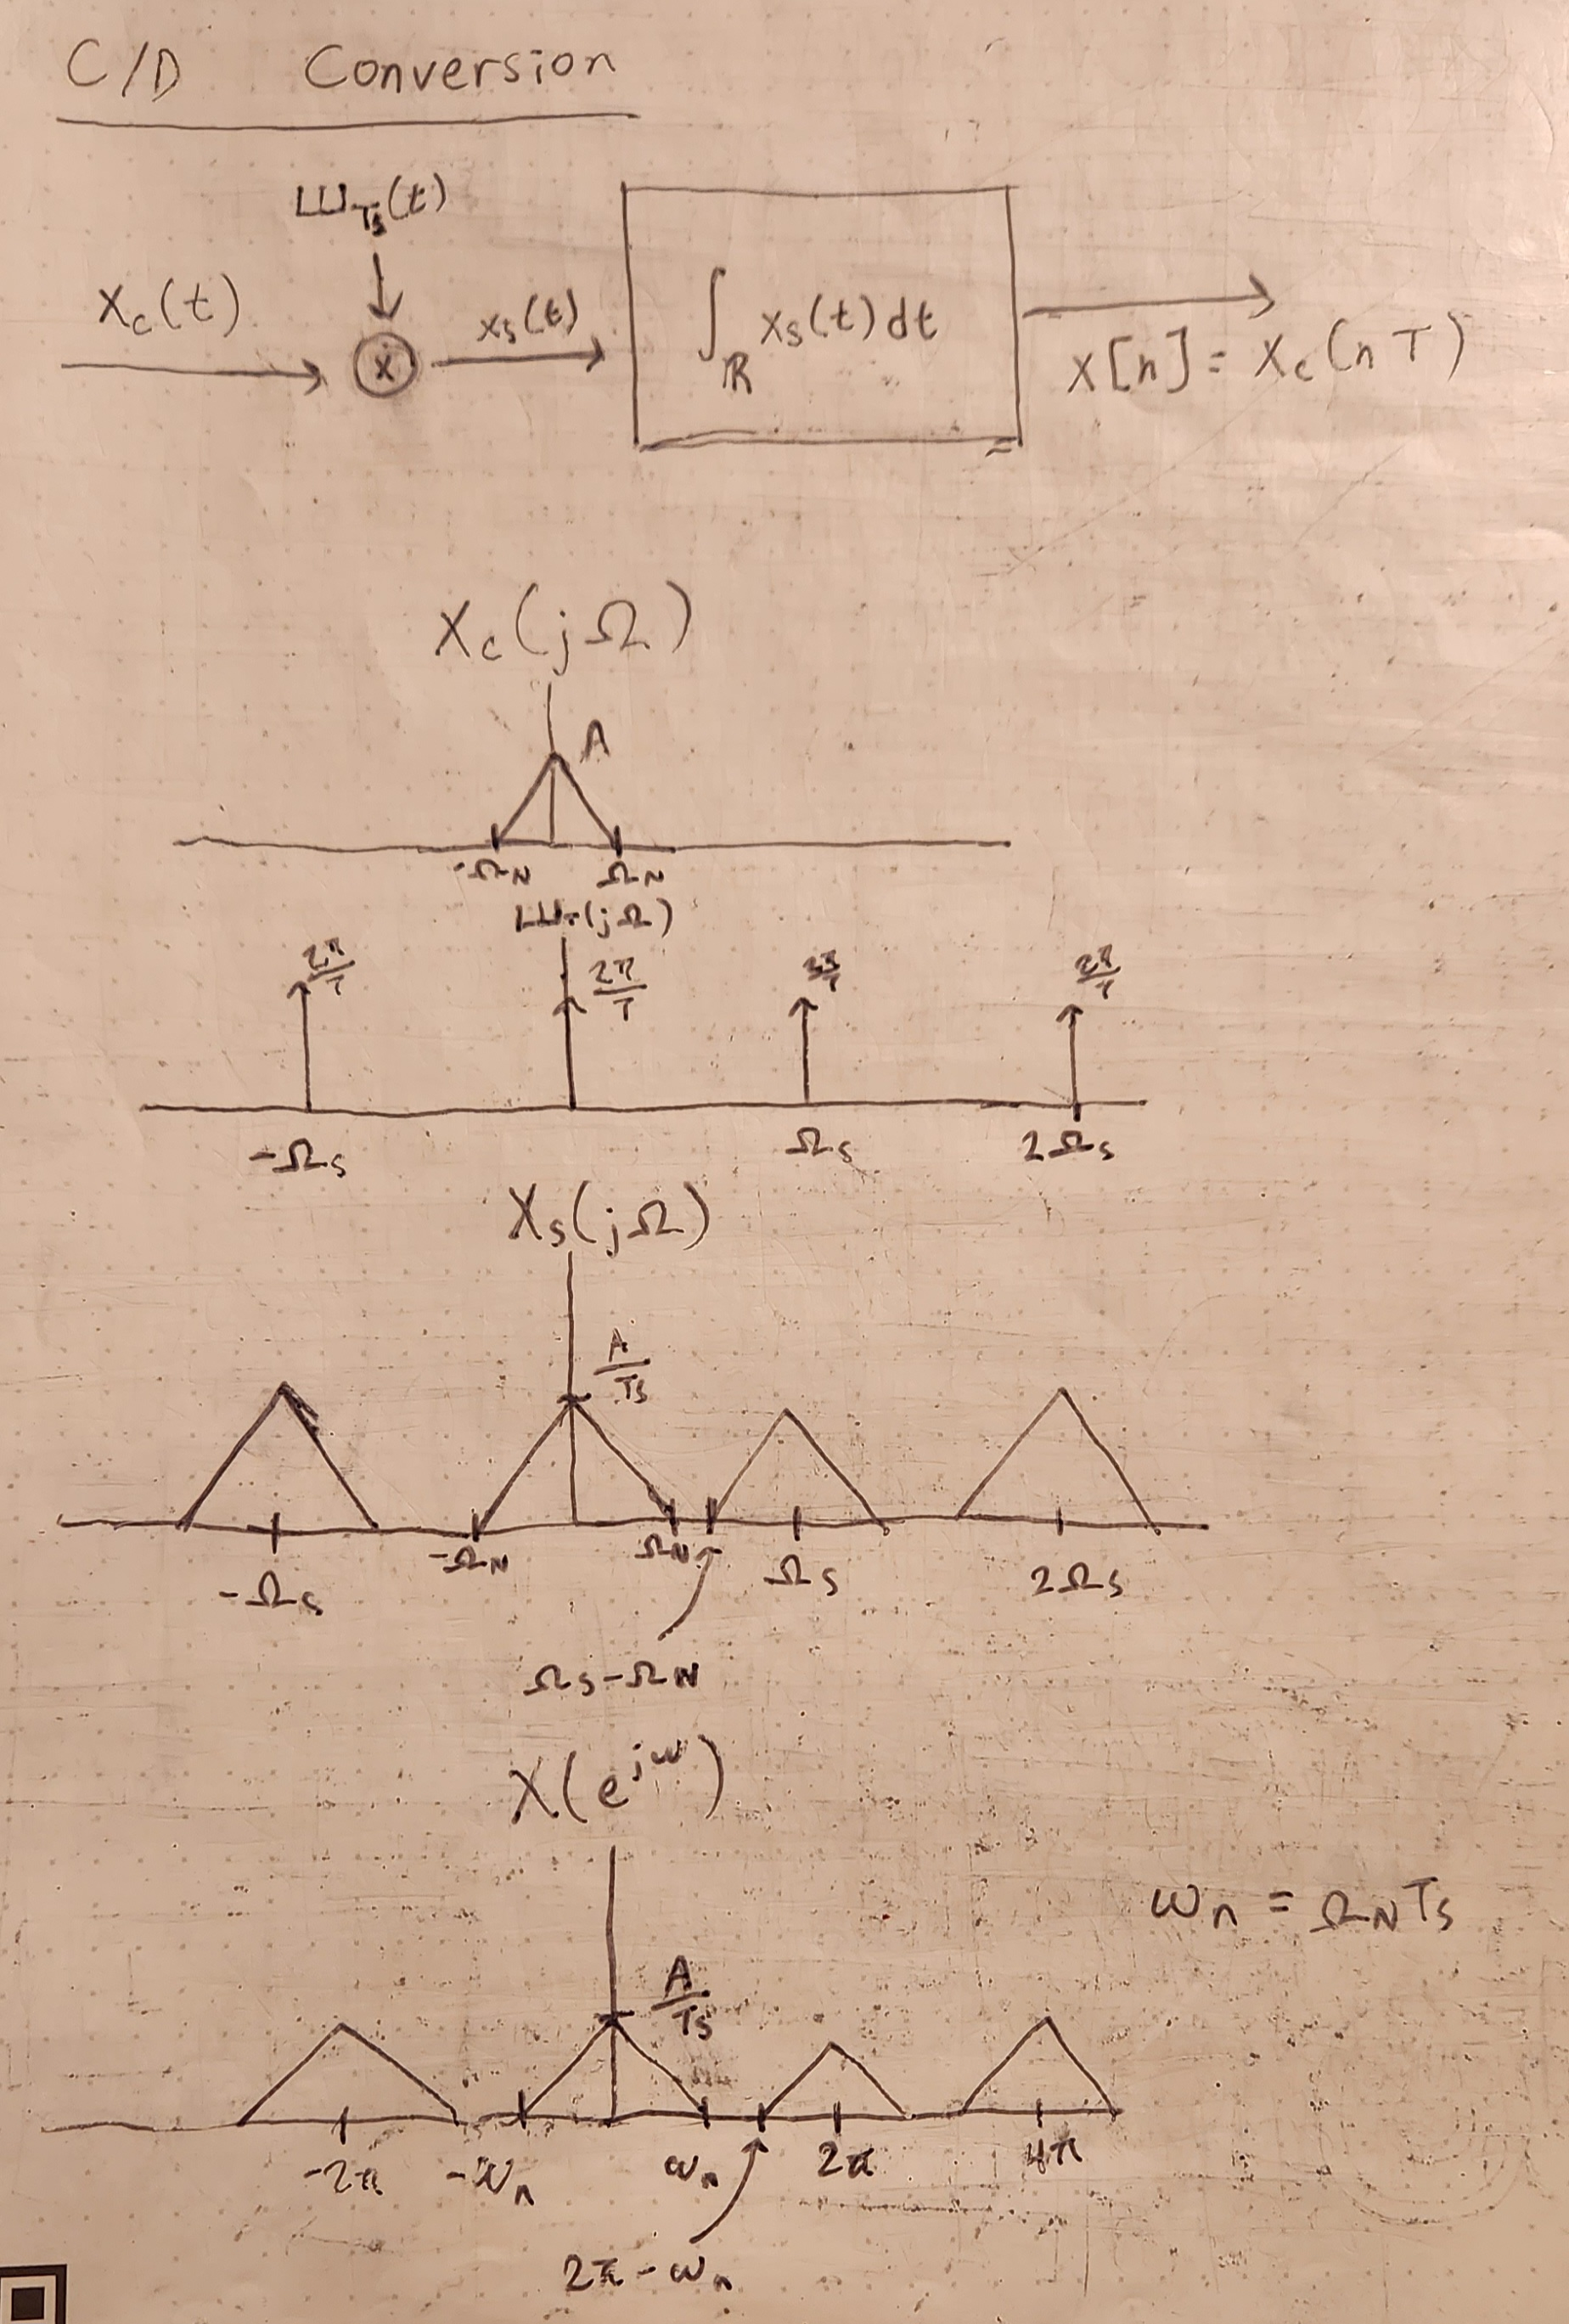
\includegraphics[scale=0.165]{graphics/cd_conversion.jpg}

  \pagebreak

  \subsubsection{D/C Conversion}

  \small\textbf{Mismatch in Reconstruction and Sampling Period}:

  Assuming no aliasing effects, if \(T_r \neq T_s\)

  \(y_r(t) = \dfrac{T_r}{T_s}x_c\prn{\dfrac{T_s}{T_r}t}\)

  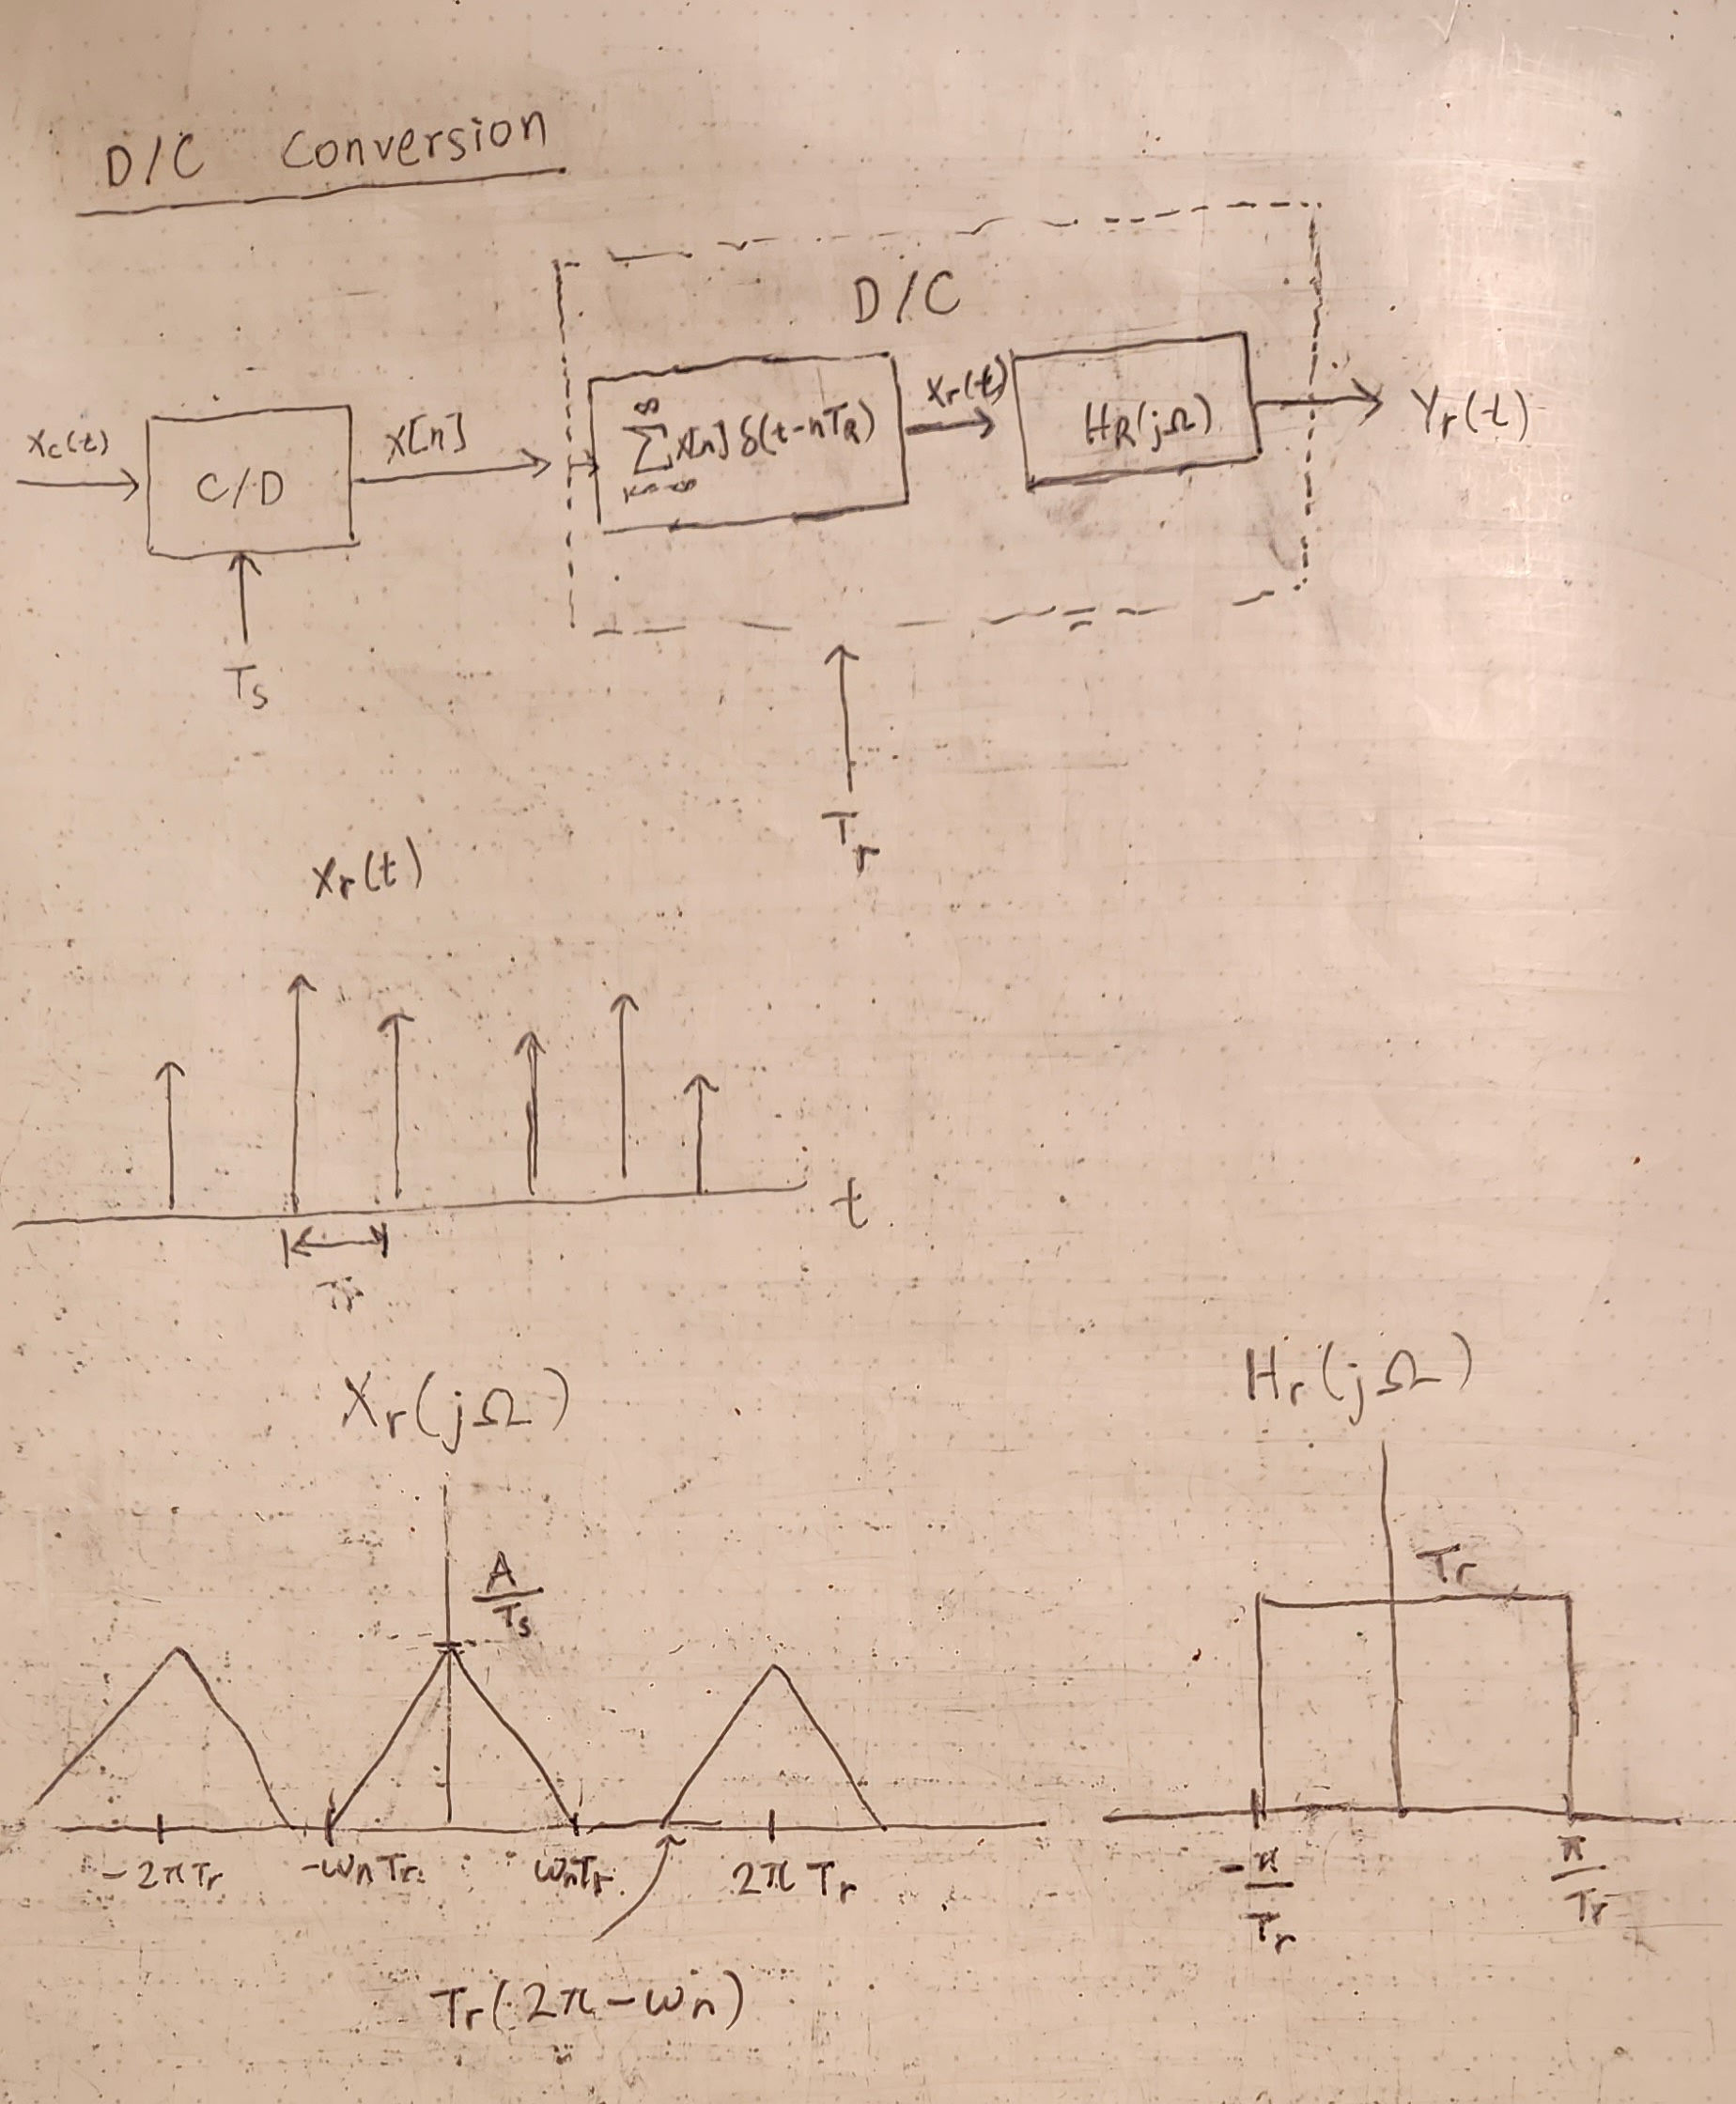
\includegraphics[scale=0.2]{graphics/dc_conversion.jpg}

  \pagebreak

  \subsubsection{Compression and Decimation}

  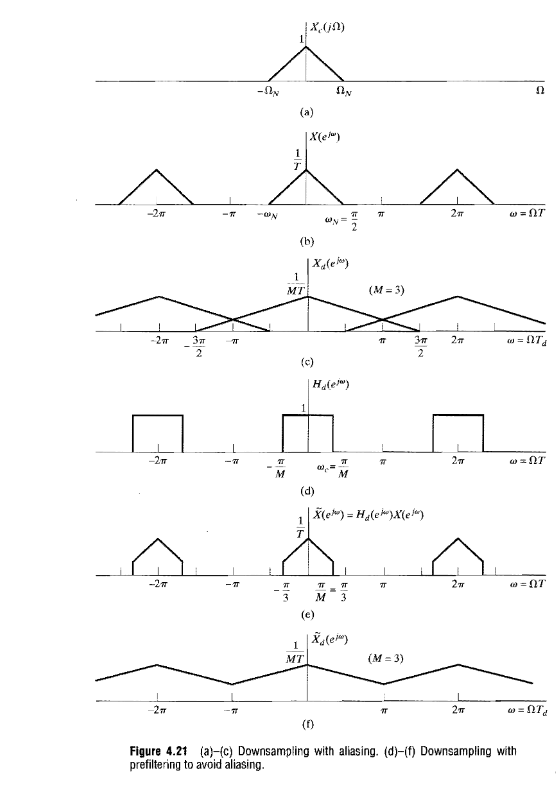
\includegraphics[scale=0.7]{graphics/downsampling.png}

  \pagebreak

  \subsubsection{Expansion and Interpolation}

  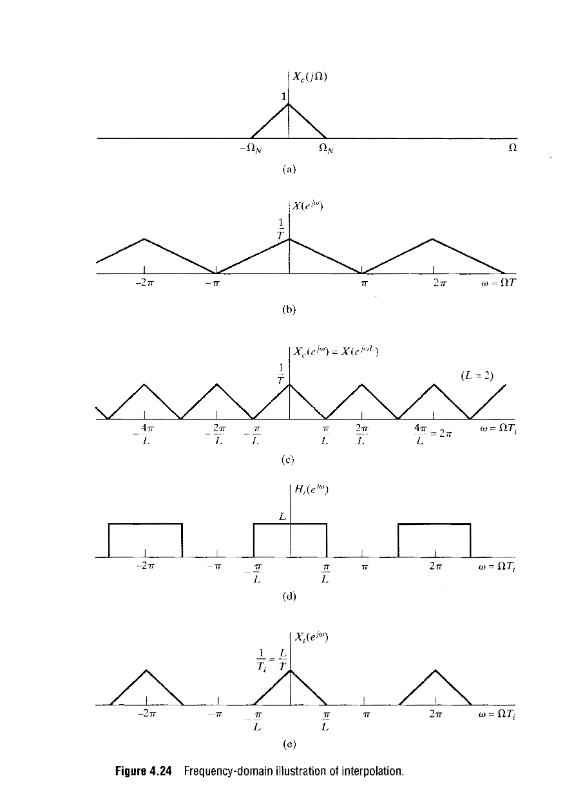
\includegraphics[scale=0.7]{graphics/upsampling.png}

  \pagebreak

  \subsubsection{Change Sampling Rate by Noninteger Factor}

  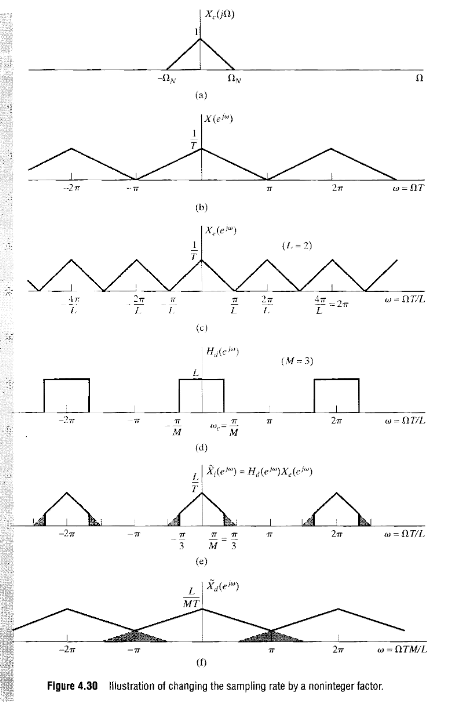
\includegraphics[scale=0.7]{graphics/noninteger.png}

  \pagebreak

  \subsubsection{Polyphase Decompositions}

  \textbf{Noble Identities:}

  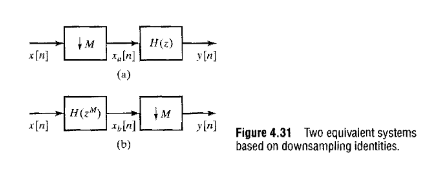
\includegraphics[scale=0.7]{graphics/compressor_noble.png}

  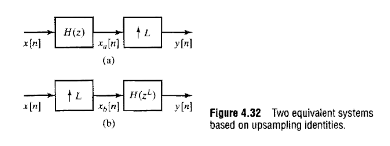
\includegraphics[scale=0.75]{graphics/expander_noble.png}

  \textbf{Polyphase Decomposition for Compression}:

  In the below diagram \(e_{k}[n] = h[nM + k]\)

  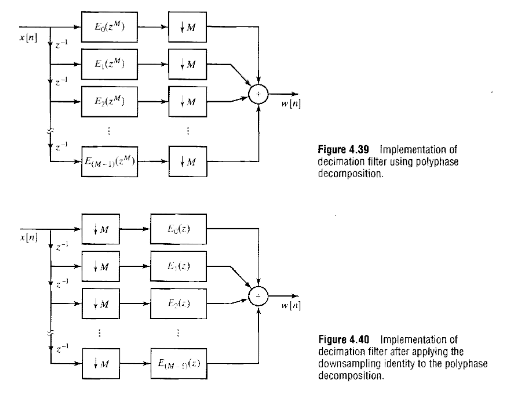
\includegraphics[scale=0.82]{graphics/polyphase_down.png}

\end{document}
